\documentclass[11pt]{beamer}

\usetheme[progressbar=frametitle]{metropolis}
\usepackage{appendixnumberbeamer}
\usepackage{FiraSans}
\usepackage{textcomp} %% put this in your preamble
\usepackage{graphicx} 
\usepackage{booktabs}
\usepackage[scale=2]{ccicons}
\usepackage{adjustbox}
\usepackage{soul}
\usepackage{caption}
	\captionsetup[figure]{	labelformat=empty, 
					font=scriptsize,
					labelfont=scriptsize, 
					justification=raggedleft}

\usepackage{pgfplots}
\usepgfplotslibrary{dateplot}



\usepackage{xspace}
\newcommand{\themename}{\textbf{\textsc{metropolis}}\xspace}

\title{Barriers to a summer fire regime in northern prairies }
\subtitle{Ecological, physical, and social}
\date{}
\author{Devan Allen McGranahan } 
\institute{\emph{Research Rangeland Management Scientist\textemdash Ecologist} \\
		     USDA Agricultural Research Service \\ 
	    	     Miles City, Montana}
    	   
		
\newcommand\blfootnotetext[1]{%
  \begingroup
  \renewcommand\thefootnote{}\footnote{#1}%
  \addtocounter{footnote}{-1}%
  \endgroup
}


\begin{document}

\maketitle

\begin{frame}{For every season: Burn, burn, burn...}
		\vspace{-3em}	
	\begin{columns}

		\begin{column}{0.5\textwidth}
			\begin{itemize} 
				\item Conventional R\textsubscript{x} fire conducted during primarily dormant season
				\item[]
				\item Increased interest in burning during non-dormant season
				\item[]
				\begin{itemize}
					\item Awareness of pre-colonial fire regimes
					\item Diversify management
				\end{itemize}
				
			\end{itemize}
			
		\end{column}
		\begin{column}{0.5\textwidth}  
			\begin{center}
				\begin{figure}
					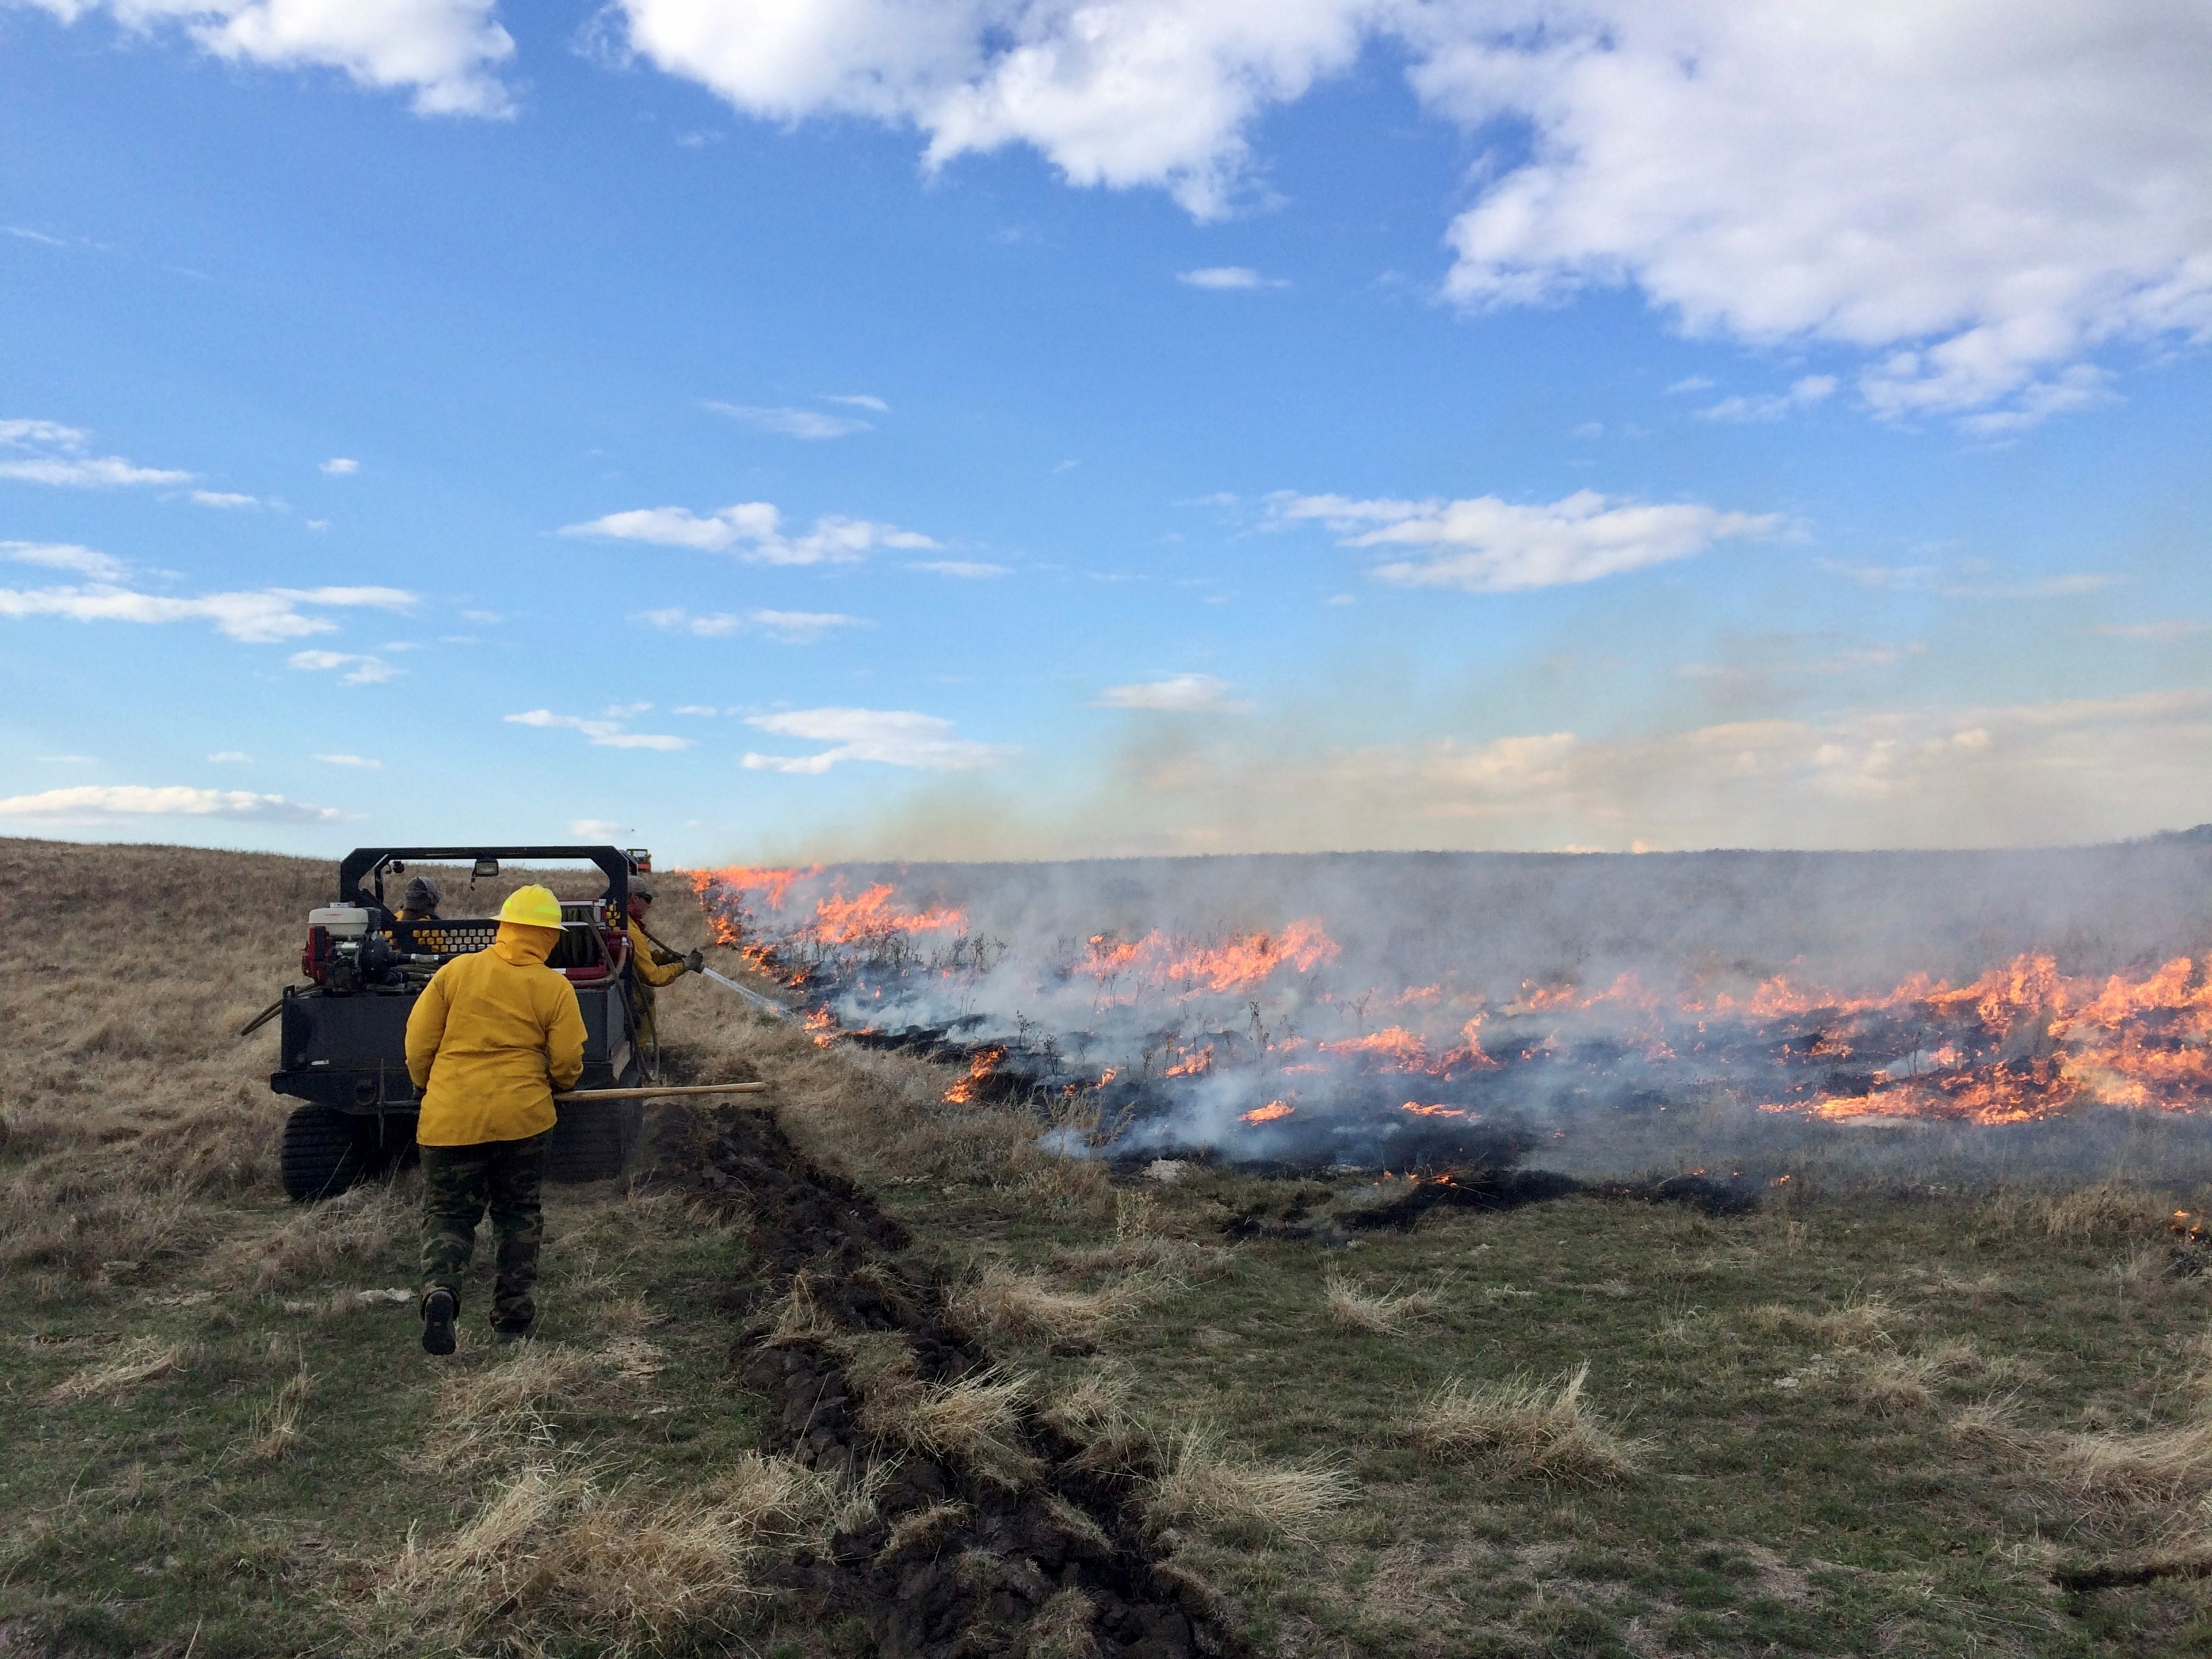
\includegraphics[width=1\linewidth]{figs/StreeterRxFire} 
					
				\end{figure}
			\end{center}
		\end{column}
	\end{columns}

	%\alert{As with most components of fire regime, \textbf{seasonality is a construct}}
\end{frame}

\begin{frame}{For every season: Burn, burn, burn...}
	
	\begin{columns}
		\begin{column}{0.5\textwidth}
			\begin{itemize} 
				\item Conventional R\textsubscript{x} fire conducted during primarily dormant season
				\item[]
				\item Increased interest in burning during non-dormant season
				\item[]
				\begin{itemize}
					\item Awareness of pre-colonial fire regimes
					\item Diversify management
				\end{itemize}
				
			\end{itemize}
			
		\end{column}
		\begin{column}{0.5\textwidth}  
			\begin{center}
				\begin{figure}
					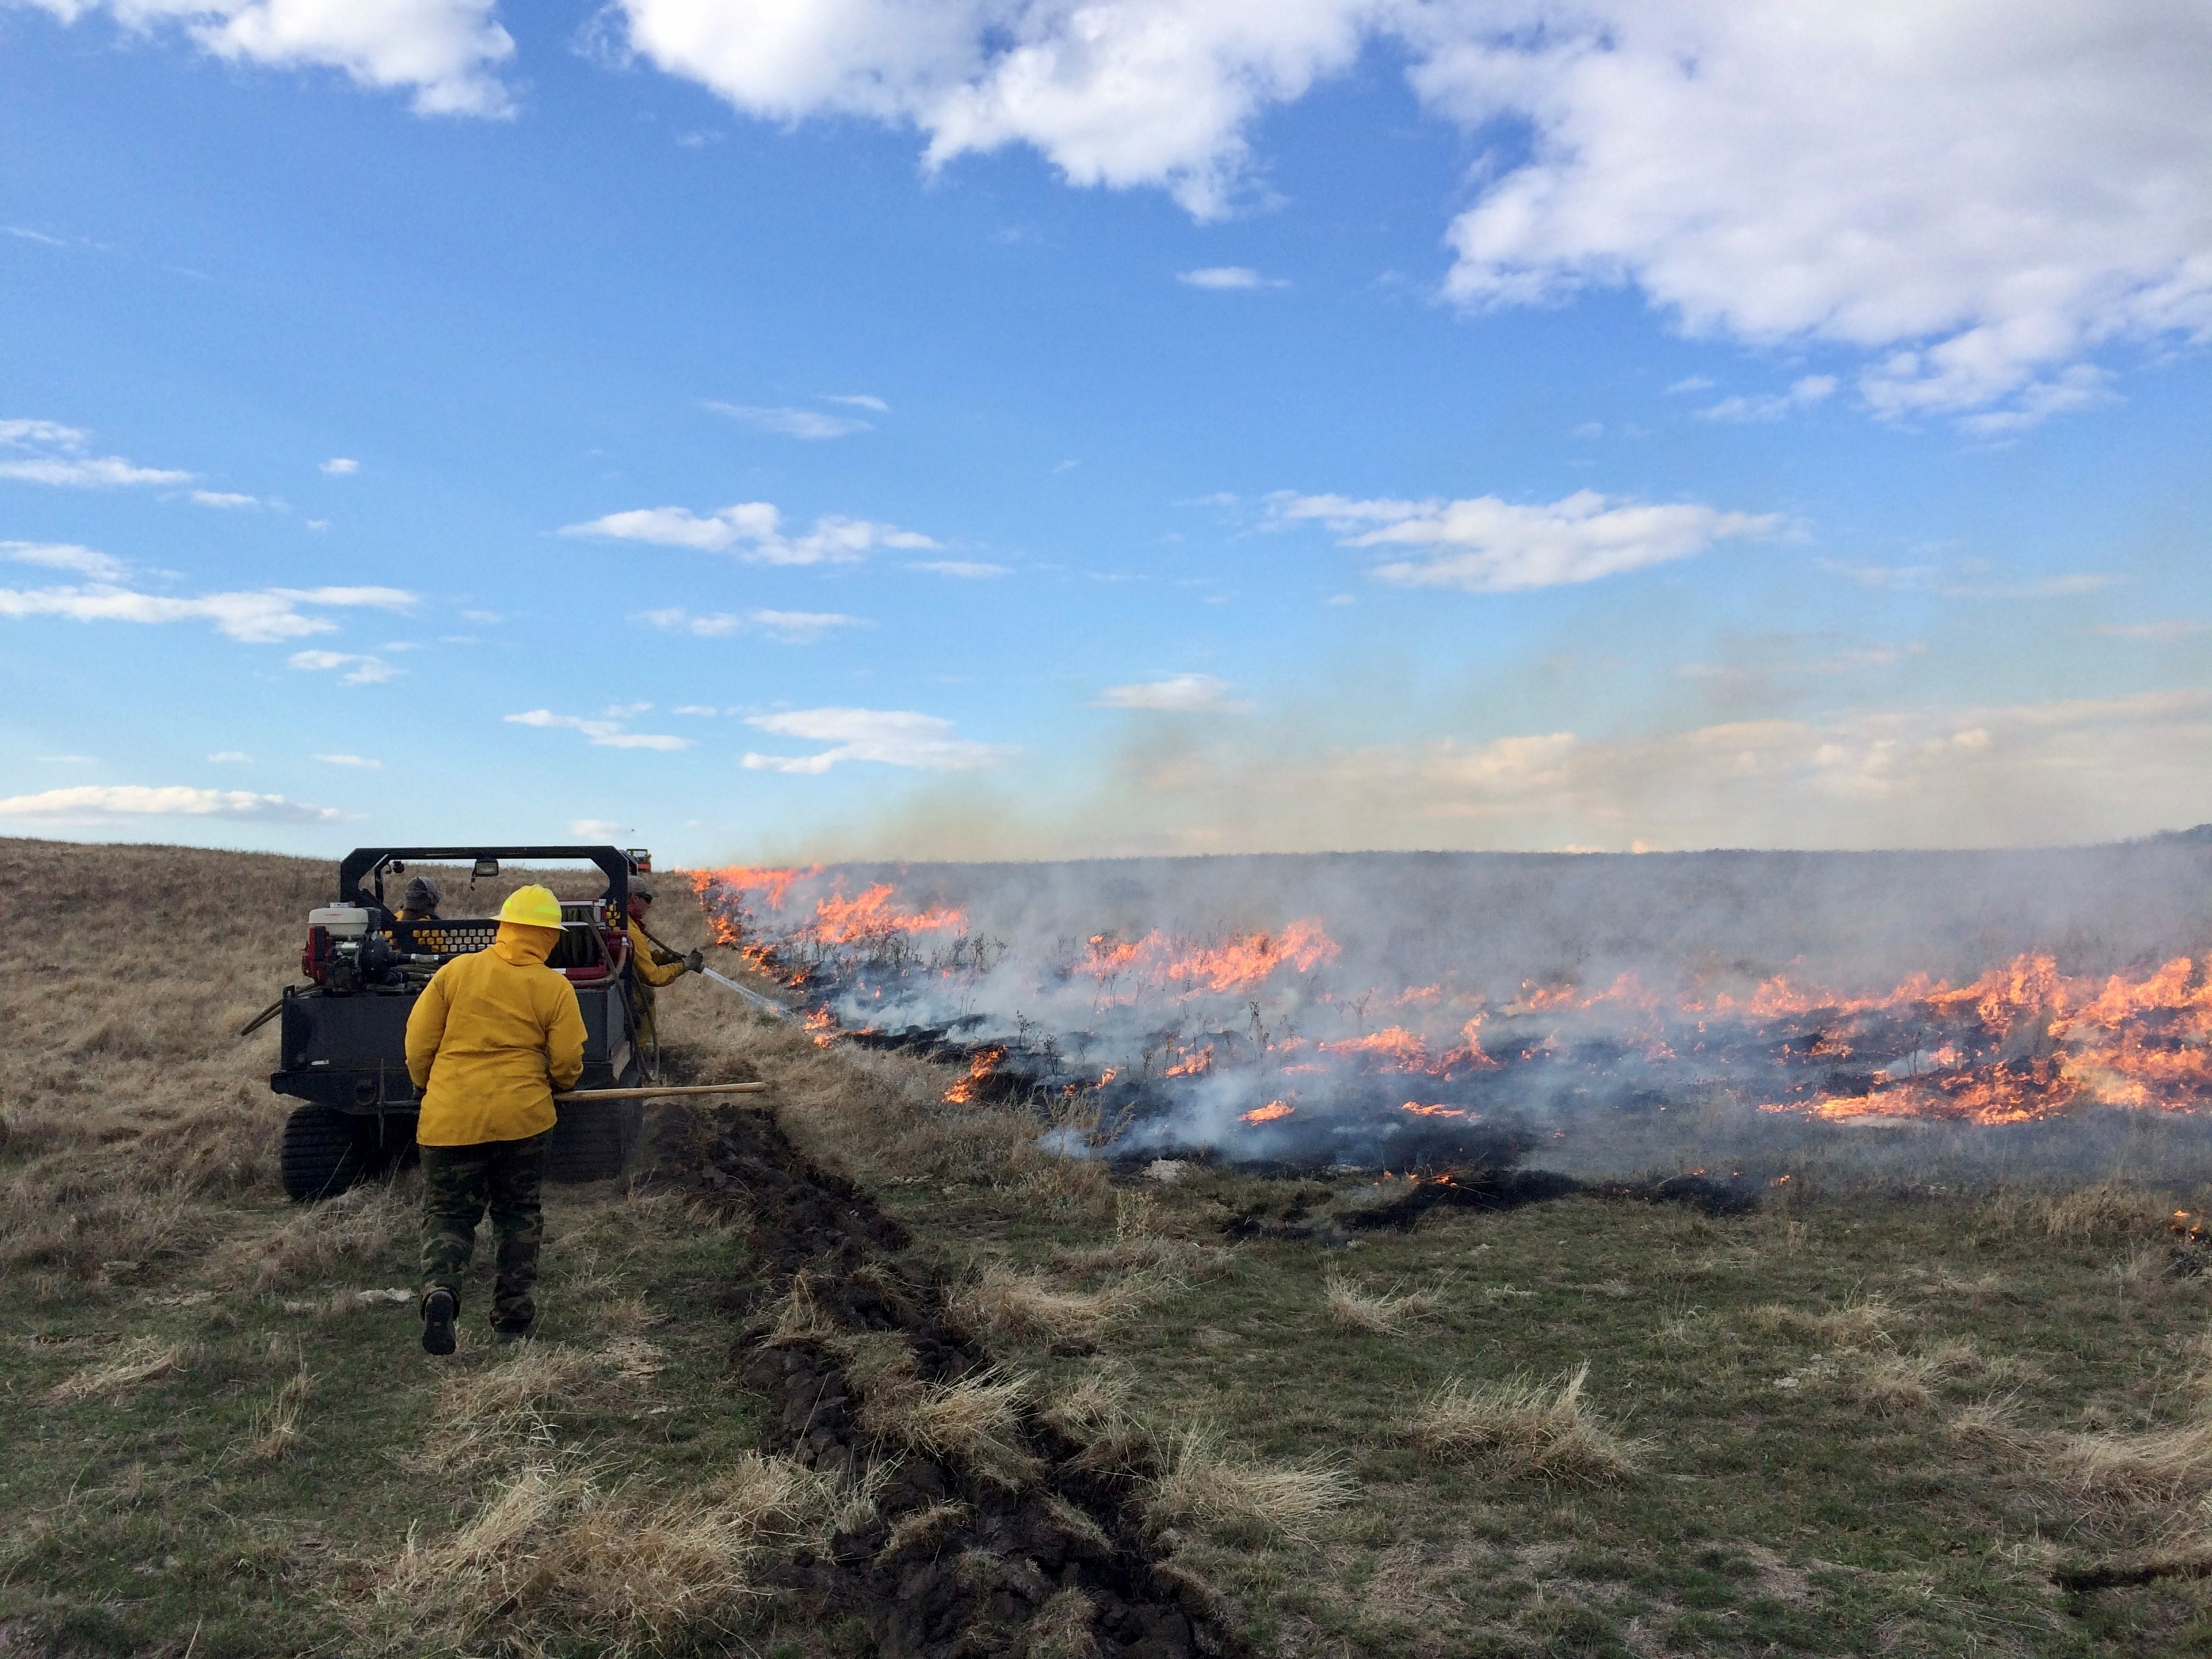
\includegraphics[width=1\linewidth]{figs/StreeterRxFire} 
					
				\end{figure}
			\end{center}
		\end{column}
	\end{columns}
\alert{As with most fire regime parameters, \textbf{seasonality is a construct}}
\end{frame}

\begin{frame}{The Western fire regime concept } 
	\begin{center}
		\begin{figure}
			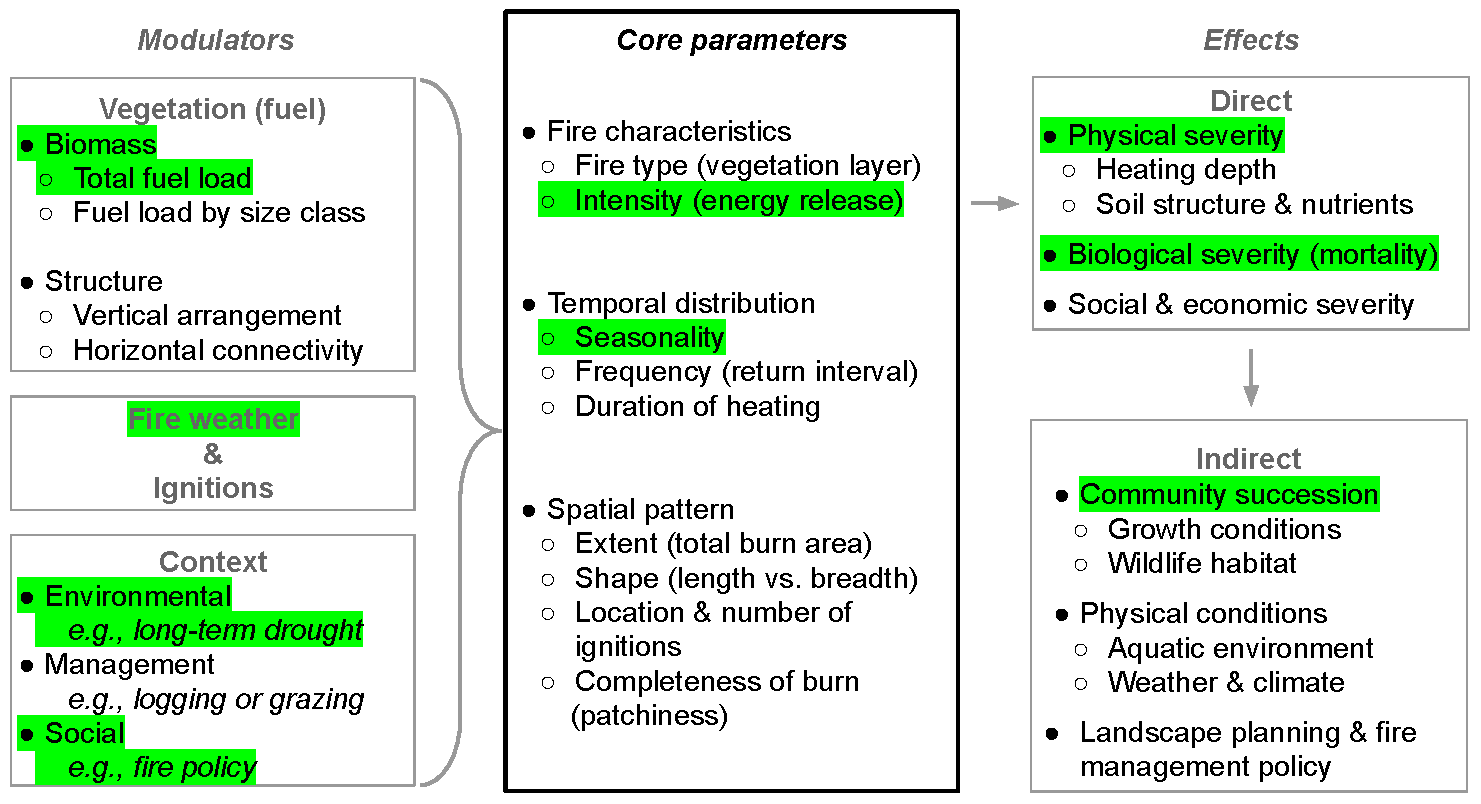
\includegraphics[width=1\linewidth]{figs/FireRegimeNAPC} 
		\end{figure}
	\end{center}
\end{frame}

\begin{frame}{Controls over fire behavior and effects}
	\begin{center}
		\begin{figure}
			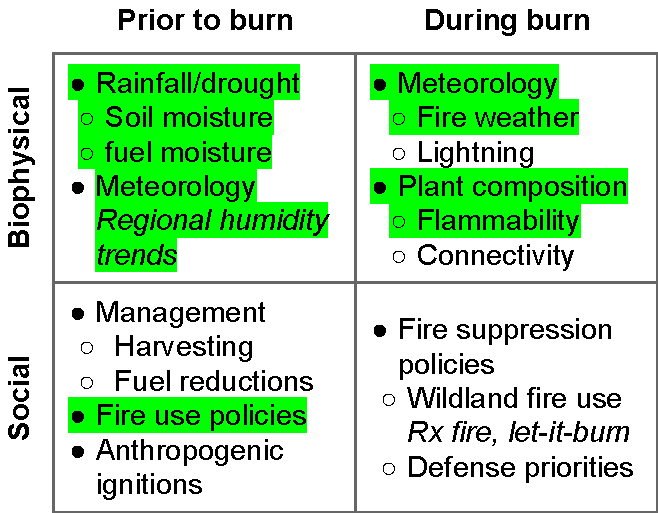
\includegraphics[width=0.9\linewidth]{figs/FireRegimeModulatorsNAPC} 
		\end{figure}
	\end{center}
\end{frame}


\begin{frame}{Case study: R\textsubscript{x} fire in the Northern Great Plains}
	\begin{center}
		\begin{figure}
			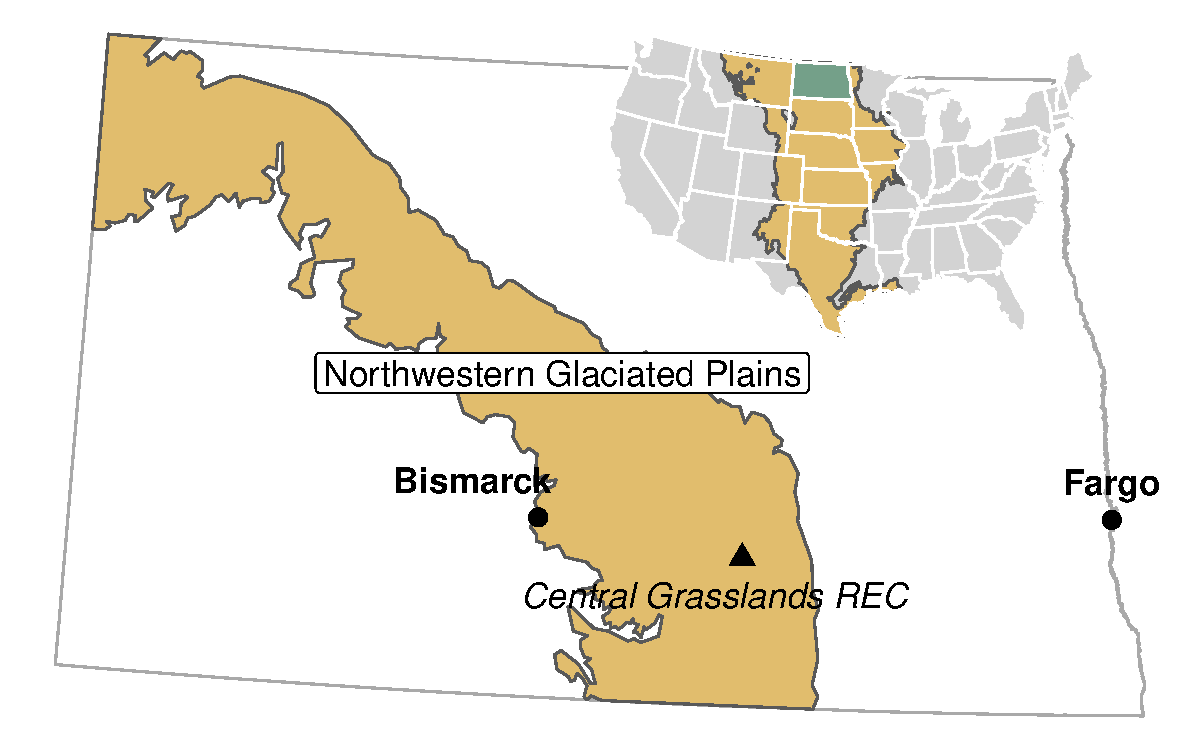
\includegraphics[width=1\linewidth]{figs/region_map-1.pdf} 
		\end{figure}
	\end{center}
\end{frame}

\begin{frame}{R\textsubscript{x} fire in the Northern Great Plains}
	\begin{center}
		\begin{figure}
			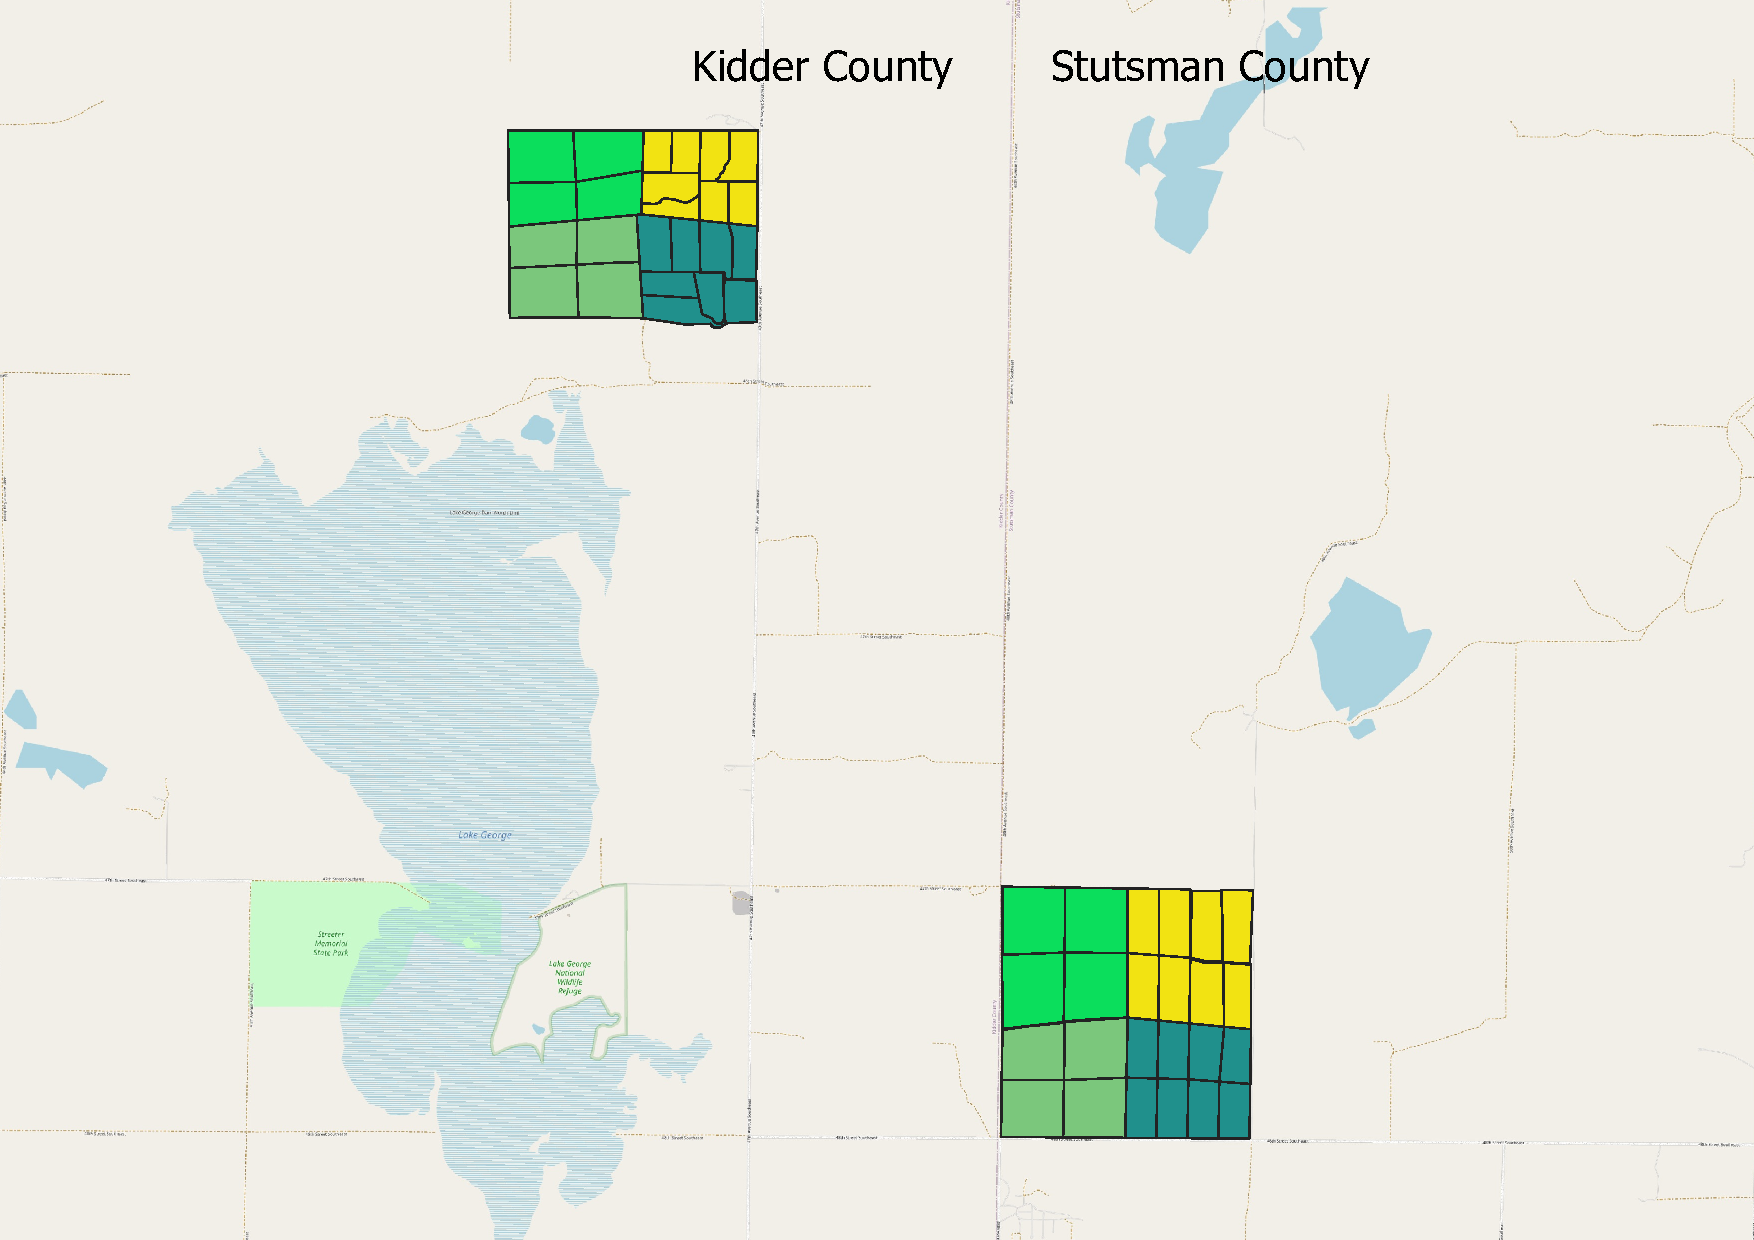
\includegraphics[width=1\linewidth]{figs/PBGmaps} 
		\end{figure}
	\end{center}
\end{frame}

\begin{frame}{Burns visible from space}
	\begin{center}
		\begin{figure}
			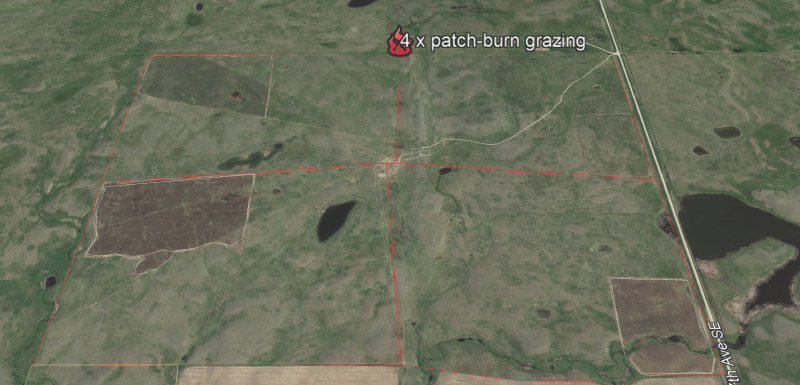
\includegraphics[width=1\linewidth]{figs/BobSWBurnedOutline2} 
		\end{figure}
	\end{center}
\end{frame}

\begin{frame}{Remotely-sensed burn severity products}
	\begin{center}
		\begin{figure}
			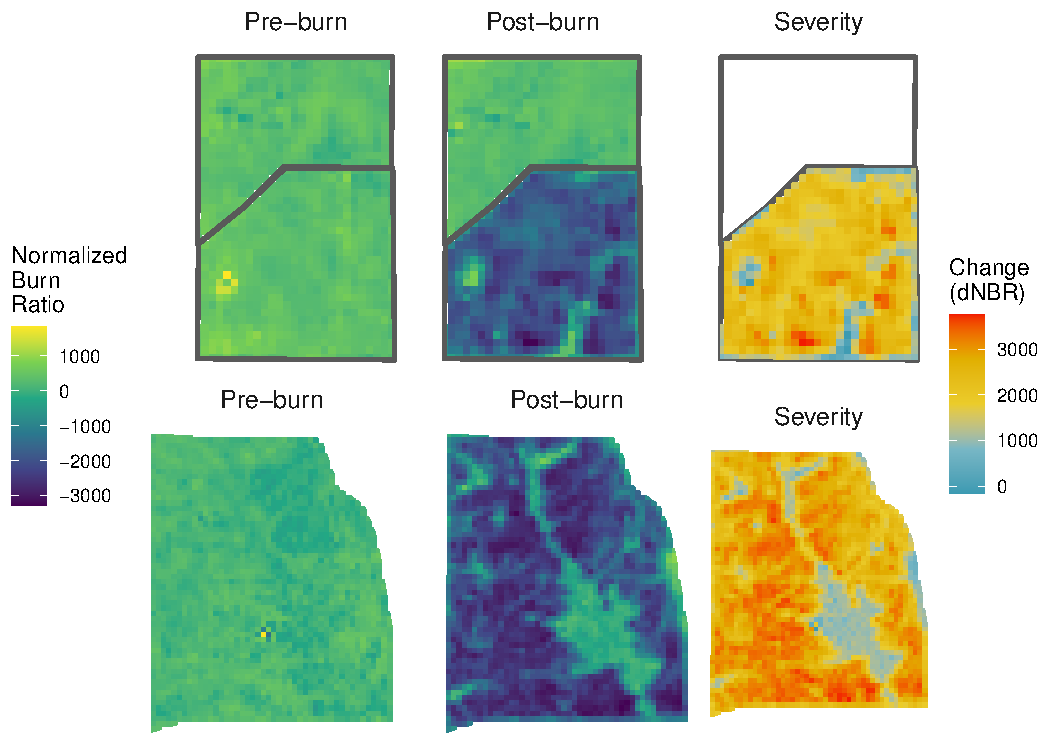
\includegraphics[width=1\linewidth]{figs/severity_gg-1} 
			\caption{An example from Dunn Ranch Prairie (McGranahan et al. 2022 \emph{Land})}
		\end{figure}
	\end{center}
\end{frame}

\begin{frame}{Spotty success in completing summer burns}

	\begin{center}
		\begin{figure}
			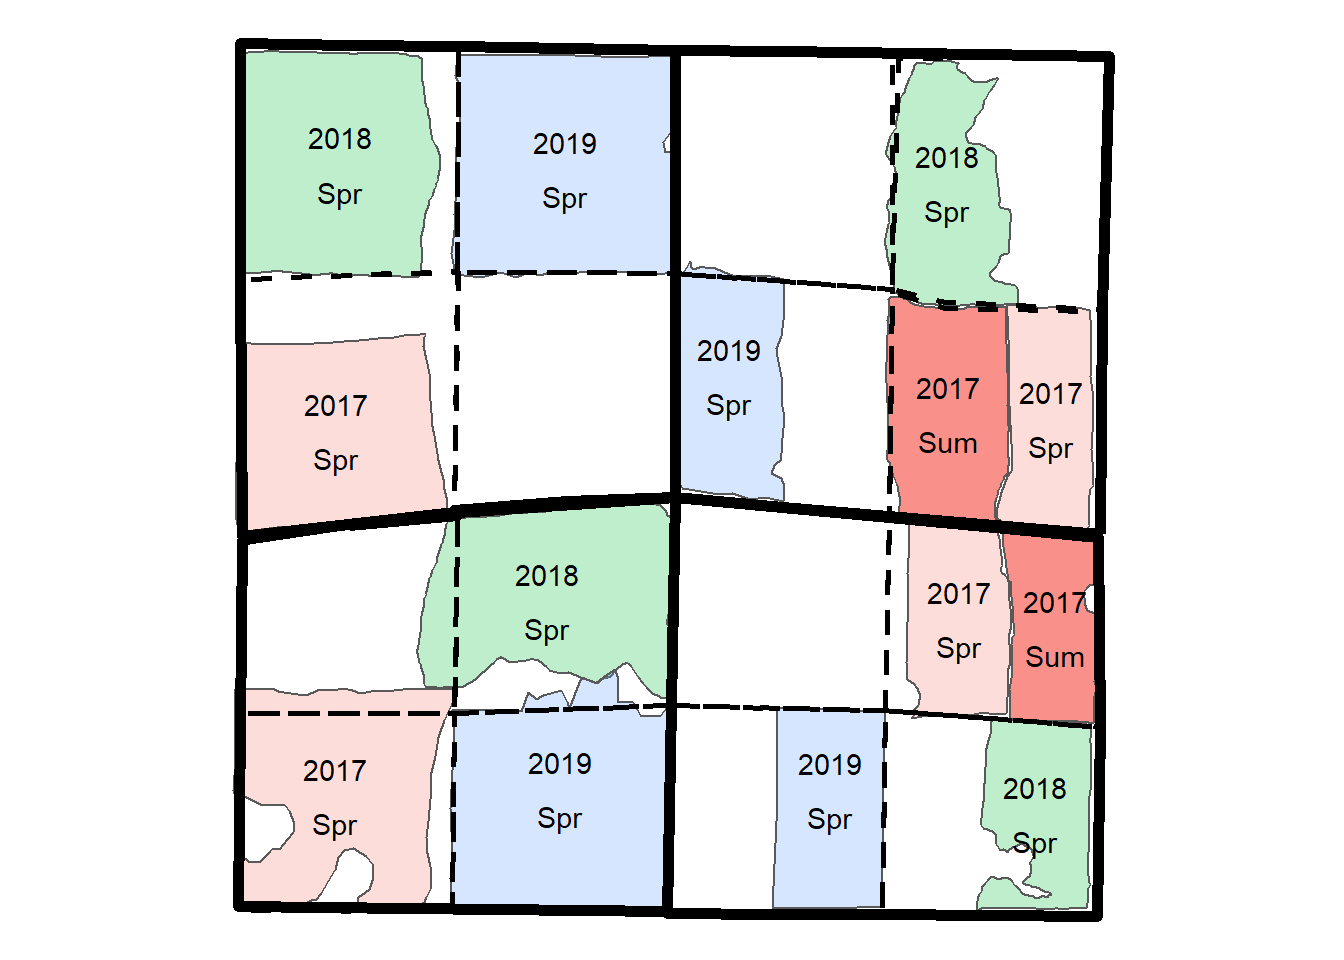
\includegraphics[width=0.9\linewidth]{figs/BarkerBurns-1} 
			\caption{2019 burn map for southern study block}
		\end{figure}
	\end{center}
\end{frame}

\begin{frame}{Barriers to summer R\textsubscript{x} fire } 
	All opportunities and limitations fit within fire regime concept
	\begin{itemize}
		\item Biophysical 
		\item[] \emph{mostly, \alert{too wet}}
		\begin{itemize}
			\item High live moisture fuel content (\emph{photosynthesis})
			\item High dead moisture fuel content (\emph{humidity})
			\item Poor convection/smoke dispersal (\emph{humidity})
		\end{itemize}
		\item[]
		\item Social 
		\item[] \emph{mostly, \alert{too dry}}
		\begin{itemize}
			\item Local burn restrictions
			\item Control issues
		\end{itemize}
	\end{itemize}
	
\end{frame}

\section{A tale of two fires}

\begin{frame}{What a difference a few days make! } 
	\begin{columns}
		\begin{column}{0.5\textwidth}
				\begin{center}
				\begin{figure}
					%\caption{5 May 2018}
					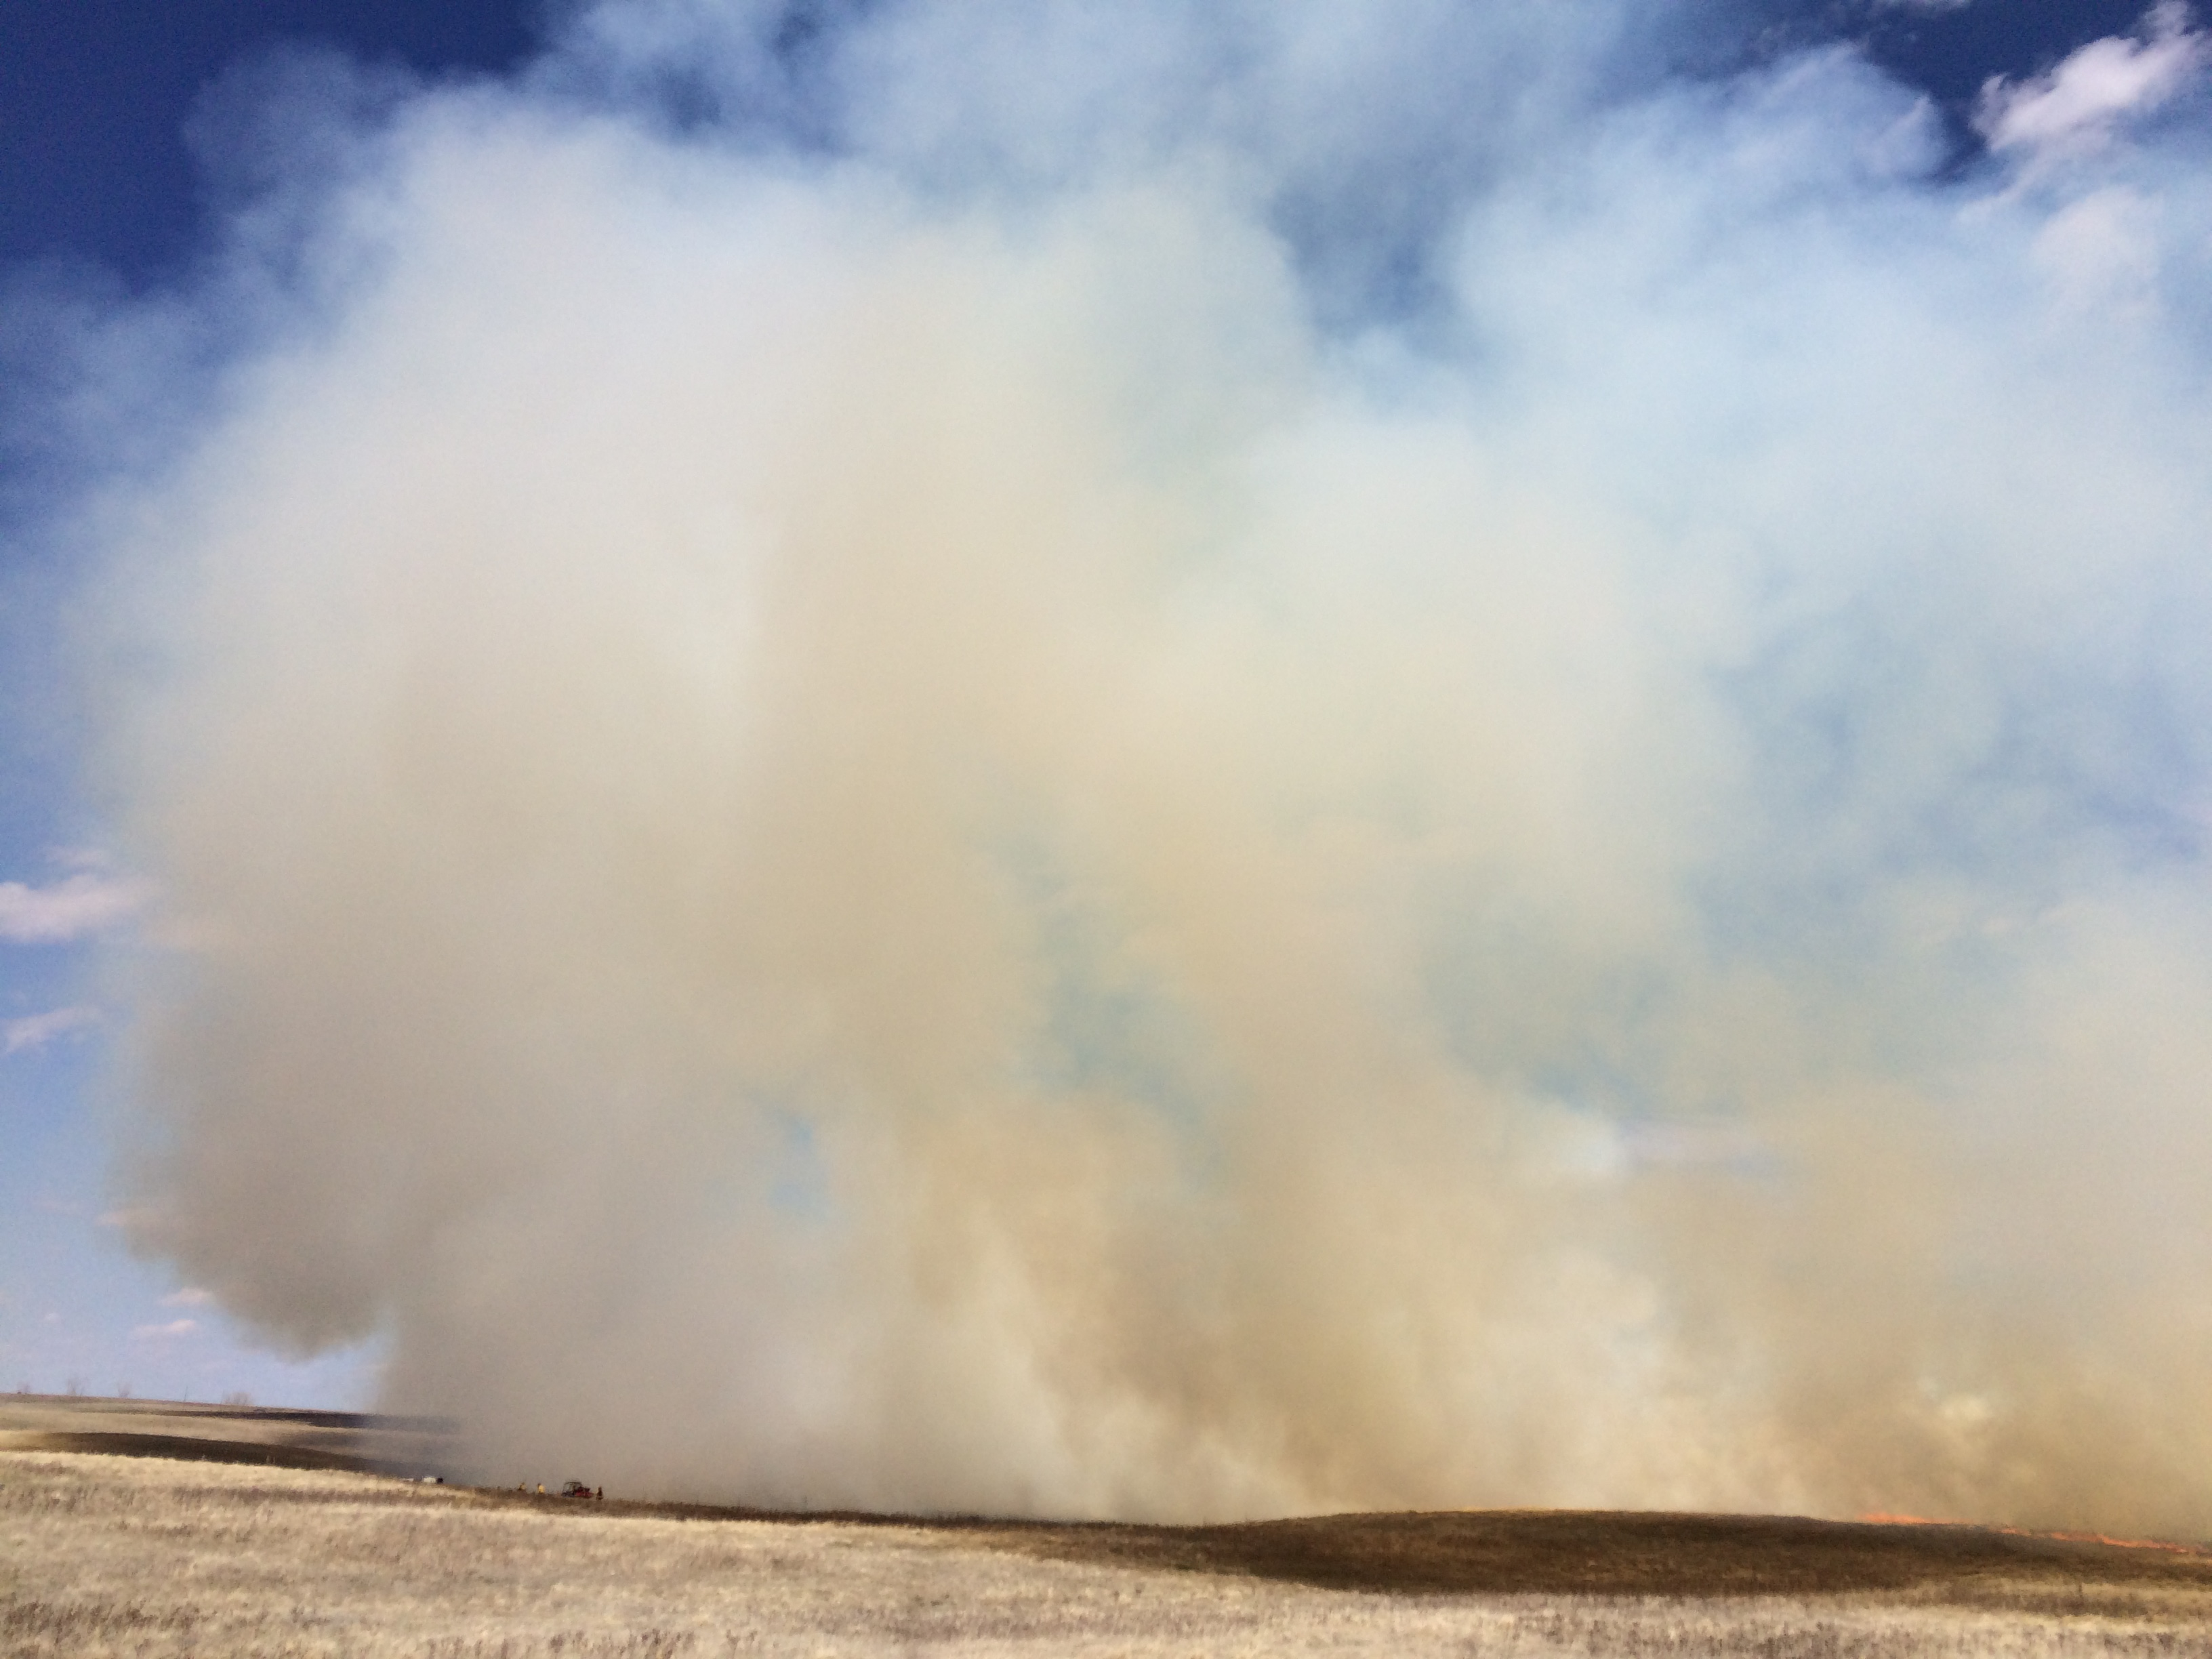
\includegraphics[width=0.9\linewidth]{figs/GoodBurn} 
				\end{figure}
			\end{center}
		\end{column}
		\begin{column}{0.5\textwidth}  
			\begin{center}
				\begin{figure}
					%\caption{16 May 2018}
					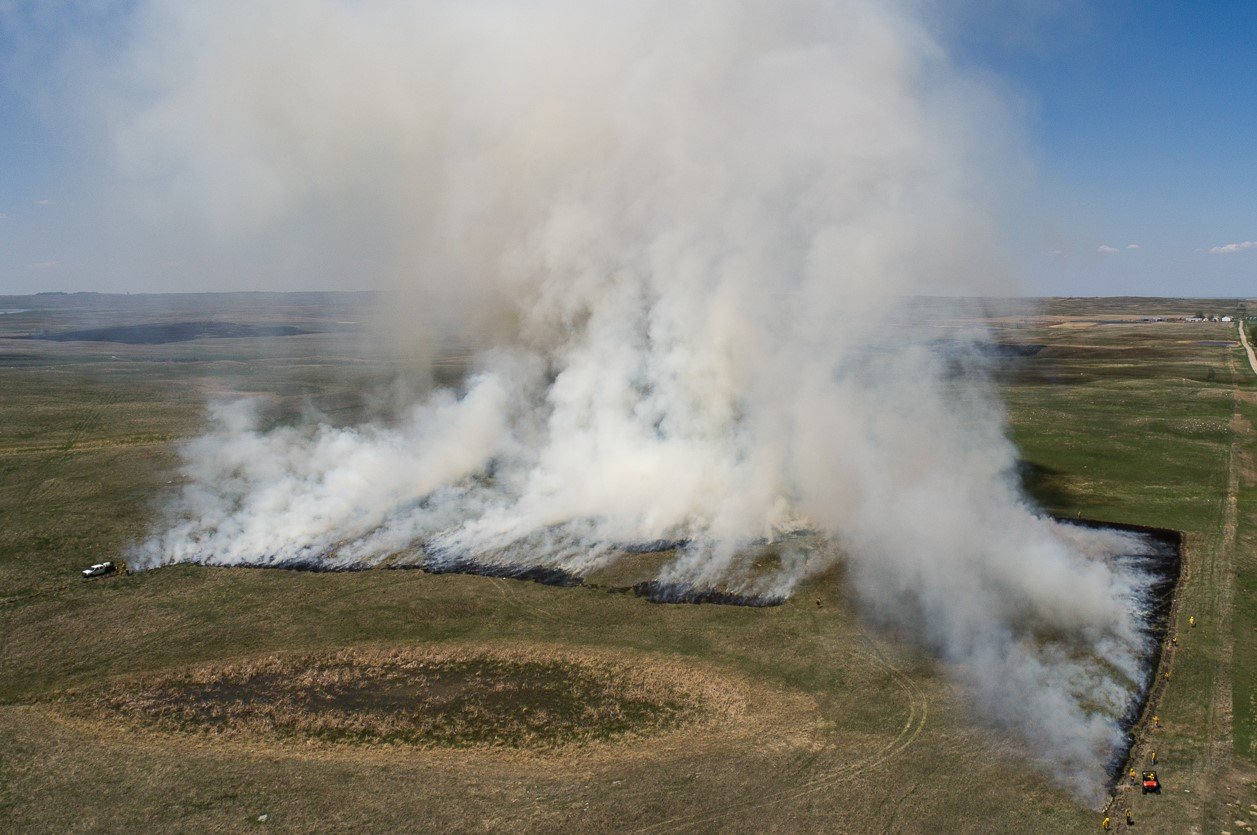
\includegraphics[width=1\linewidth]{figs/StreeterFire_17}  
				\end{figure}
			\end{center}
		\end{column}
	\end{columns}
\centering
\adjustbox{max height=\dimexpr\textheight-5.5cm\relax,
	max width=1\textwidth}{
	\begin{tabular}{ccc}
		\toprule
		5 May 2018 & \textbf{Date} & 16 May 2018 \\
		79 & \textbf{Air temp (F)} & 82 \\
		5.9 & \textbf{Wind (m s\textsuperscript{-1})} & 2.4 \\
		22 & \textbf{min RH (\%)} & 24 \\
		37 & \textbf{Dew Point (F)} & 46 \\\bottomrule
	\end{tabular}
}
\end{frame}



\section{Biophysical barriers}

\begin{frame}{The terrible, humid, green, no-good day}
	
	\begin{columns}
		\begin{column}{0.6\textwidth}
	\alert{13 August 2018}
	\begin{itemize} 
		\item Forecast called for $<~40\%$ RH by noon, but...
		\begin{itemize}
			\item 54\% at 1200
			\item 50\% at 1500
		\end{itemize}
	\item[]
		\item Modeled historical data (gridMET) says RH reached 28\%
	\item[]
		\item Local factors constrain ignition and spread
				\begin{itemize}
			\item Transpiration by green plants
			\item Humid air resists heating, lift
		\end{itemize}
		
	\end{itemize}
	
		\end{column}
		\begin{column}{0.4\textwidth}  
			\begin{center}
				\begin{figure}
					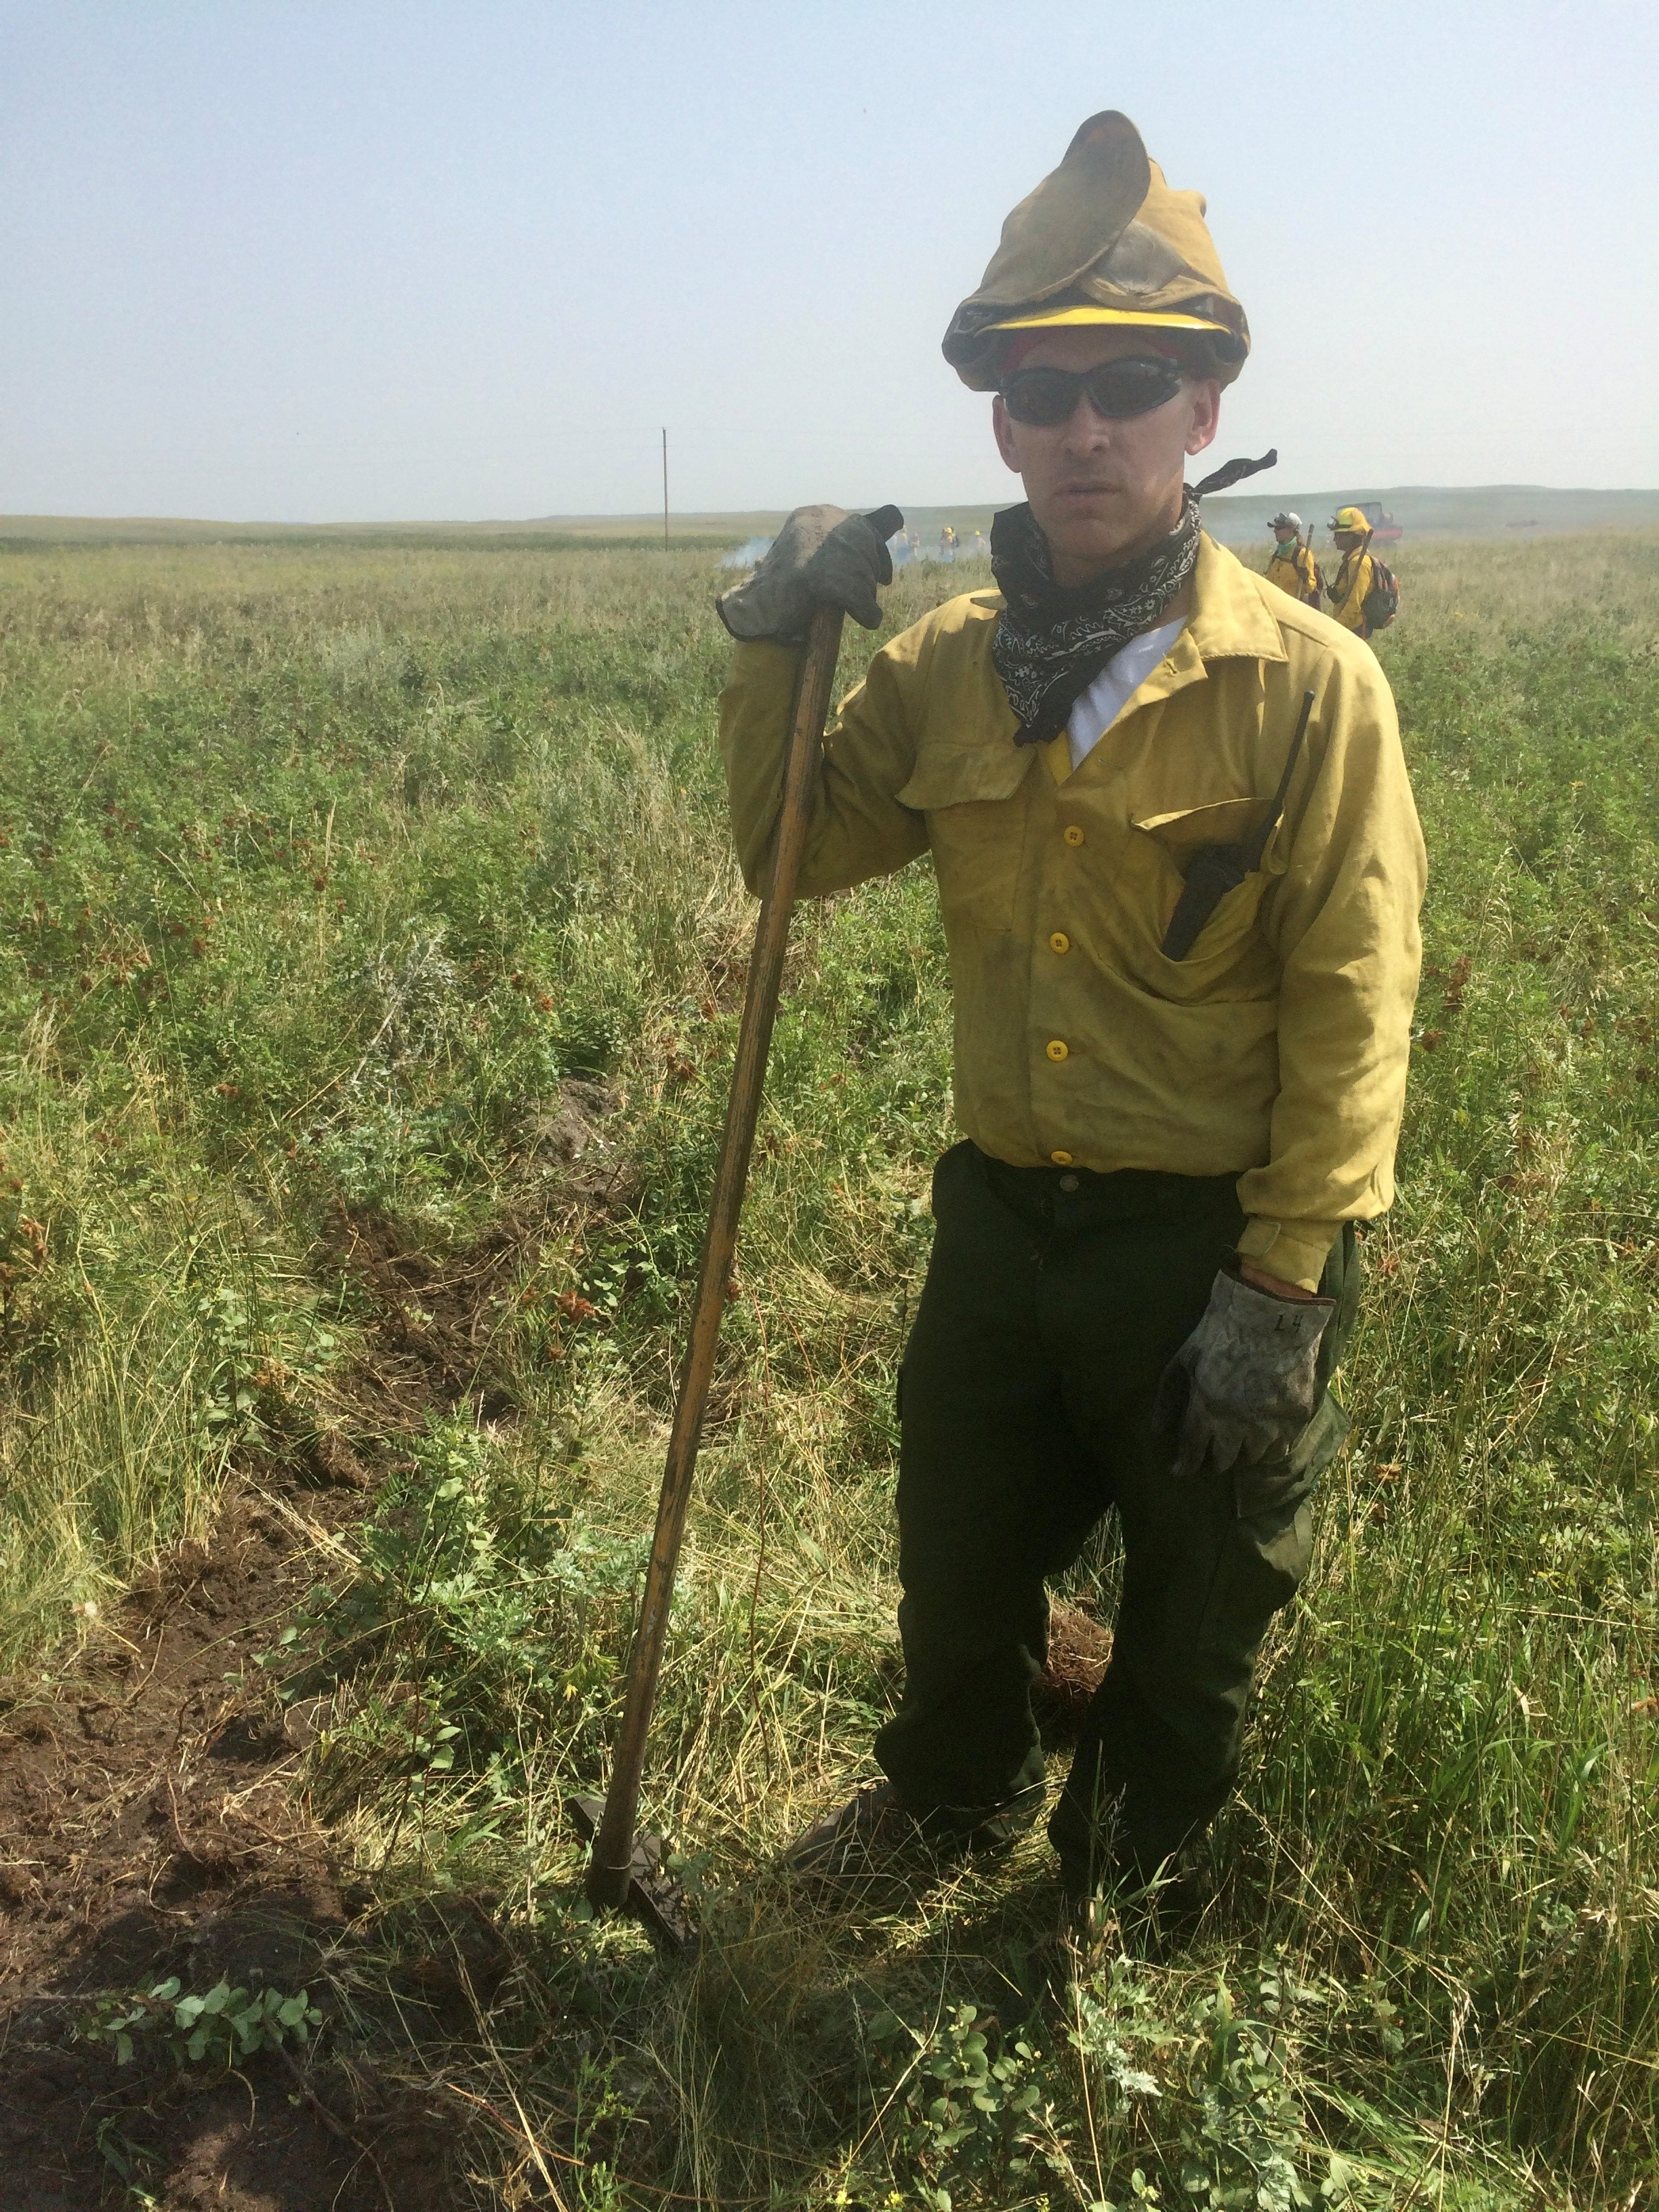
\includegraphics[width=0.9\linewidth]{figs/TorreGreenFuel} 
					
				\end{figure}
			\end{center}
		\end{column}
	\end{columns}
\end{frame}

\section{Social barriers}

\begin{frame}{County-level burn restrictions}
	\begin{center}
		\begin{figure}
			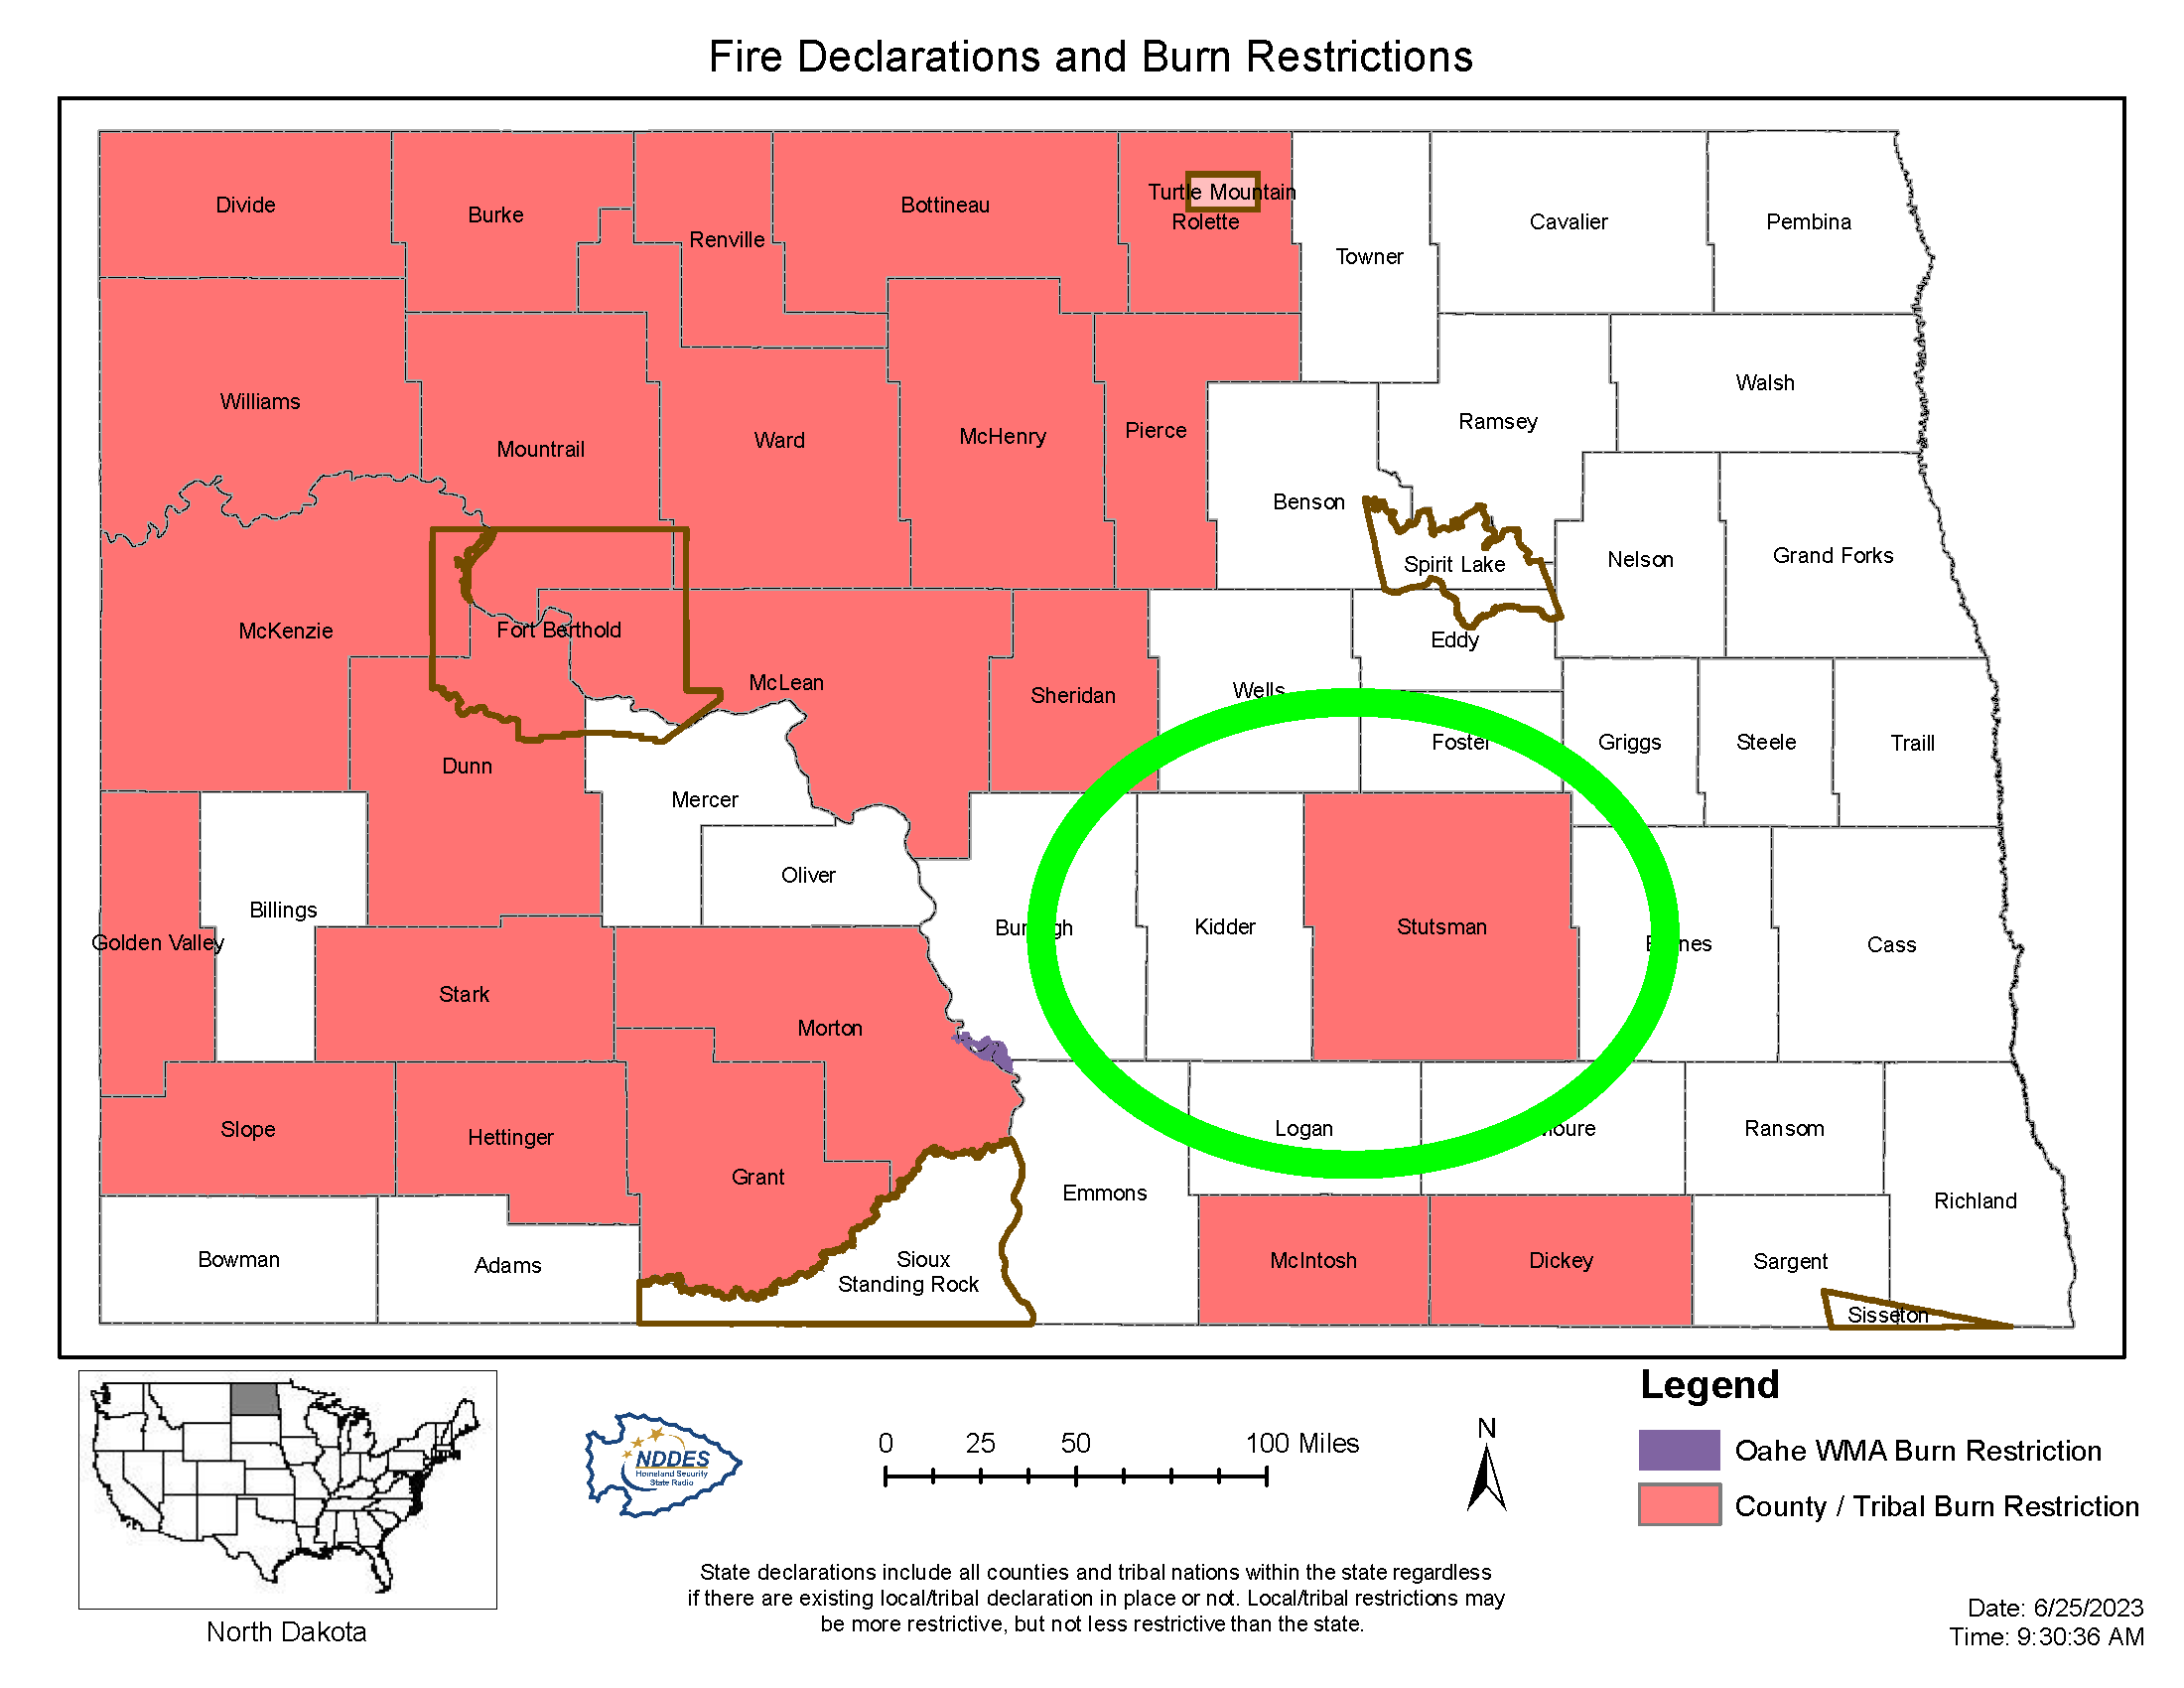
\includegraphics[width=1\linewidth]{figs/FireDeclarations.png} 
		\end{figure}
	\end{center}
\end{frame}

\begin{frame}{County-level burn restrictions}
	\begin{center}
		\begin{figure}
			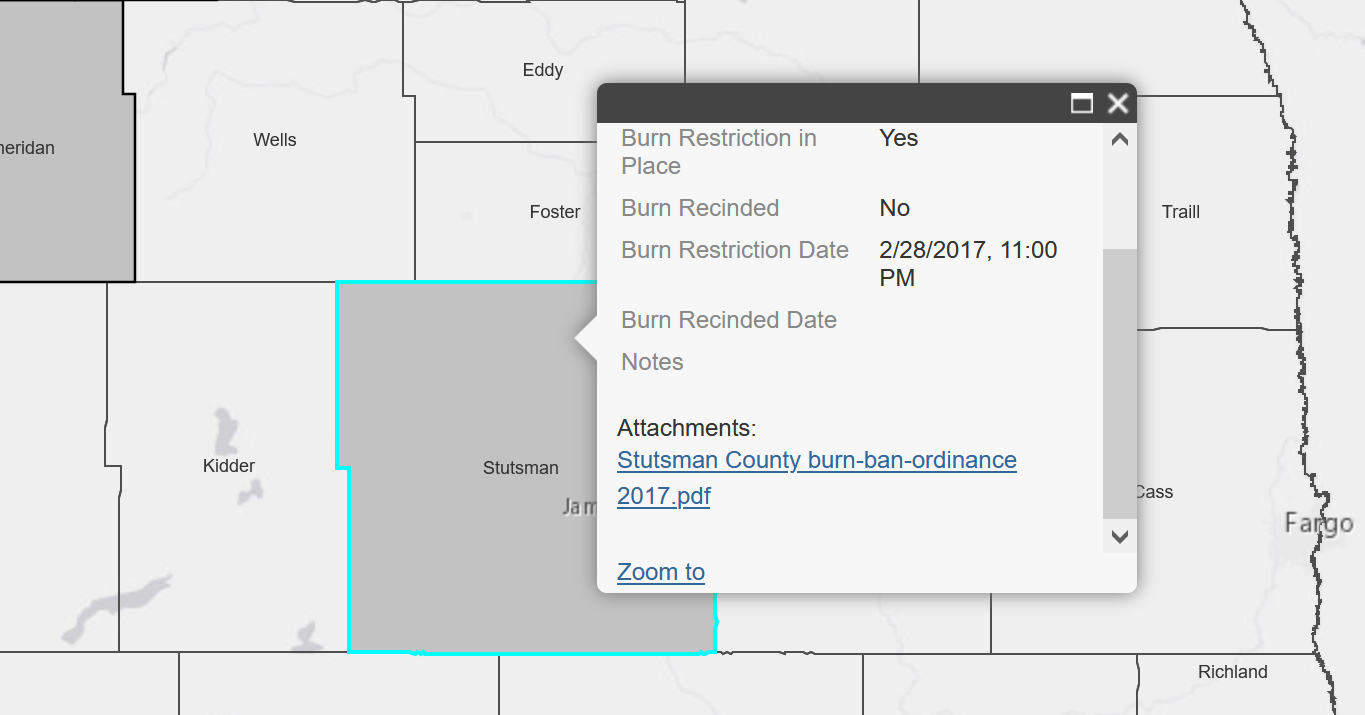
\includegraphics[width=1\linewidth]{figs/StutsmanBurnBan} 
		\end{figure}
	\end{center}
\end{frame}

\begin{frame}{Tying burn restrictions to real-time conditions}
	\begin{center}
		\begin{figure}
			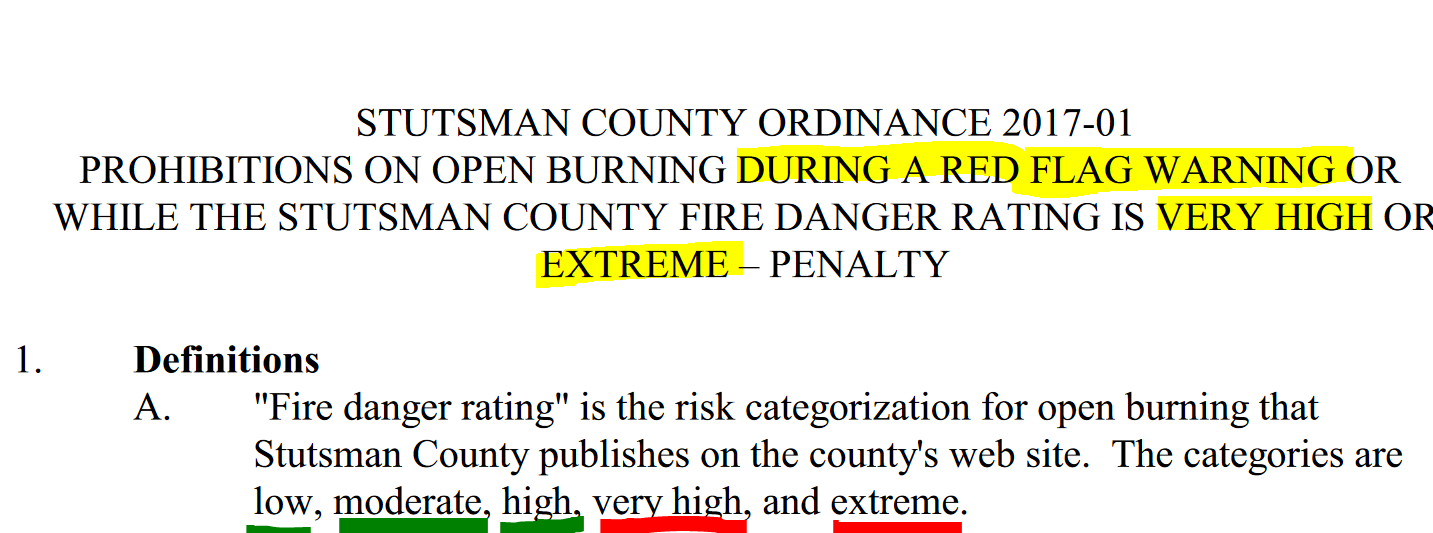
\includegraphics[width=1\linewidth]{figs/StutsmanOrdinance} 
		\end{figure}
	\end{center}
\end{frame}







\begin{frame}{Fire regime management}
	Difficult to satisfy multiple socially-constructed parameters (e.g. \emph{force patterns})
	\begin{center}
		\begin{figure}
			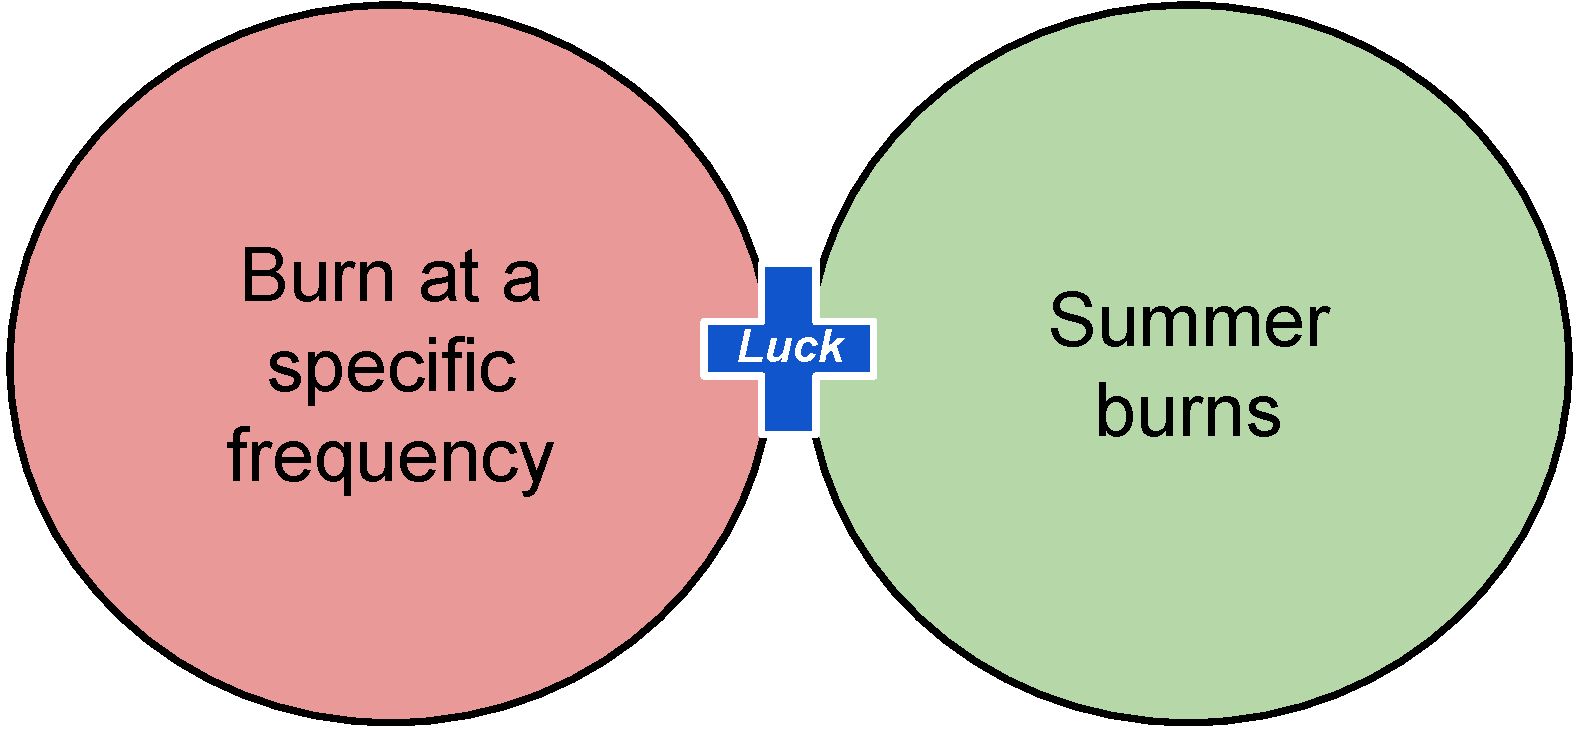
\includegraphics[width=1\linewidth]{figs/venn} 
		\end{figure}
	\end{center}
\end{frame}

\begin{frame}{Fire regime management}
	\vspace{-3em}
	Better to tweak controllable components towards desired objectives (e.g. \emph{support processes})
	\begin{center}
		\begin{figure}
			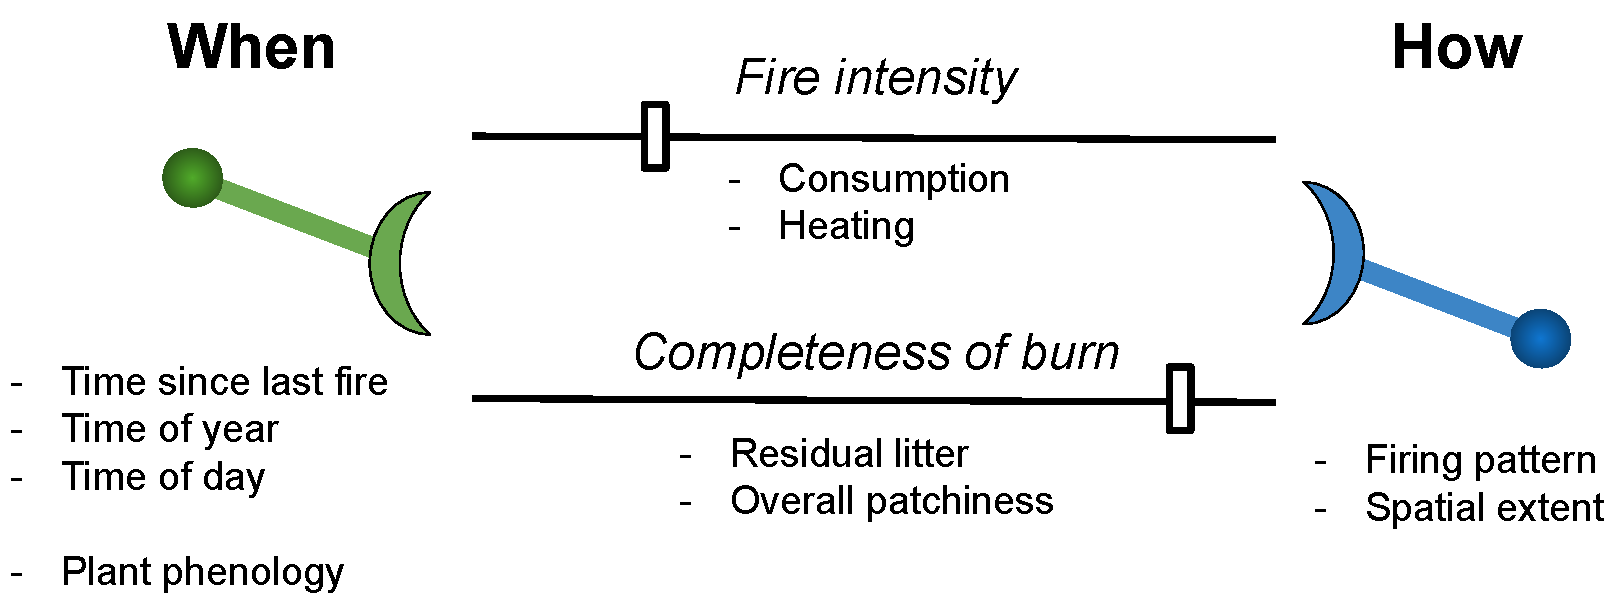
\includegraphics[width=1\linewidth]{figs/levers} 
		\end{figure}
	\end{center}
\end{frame}

\begin{frame}{Fire regime management}
	Better to tweak controllable components towards desired objectives (e.g. \emph{support processes})
	\begin{center}
		\begin{figure}
			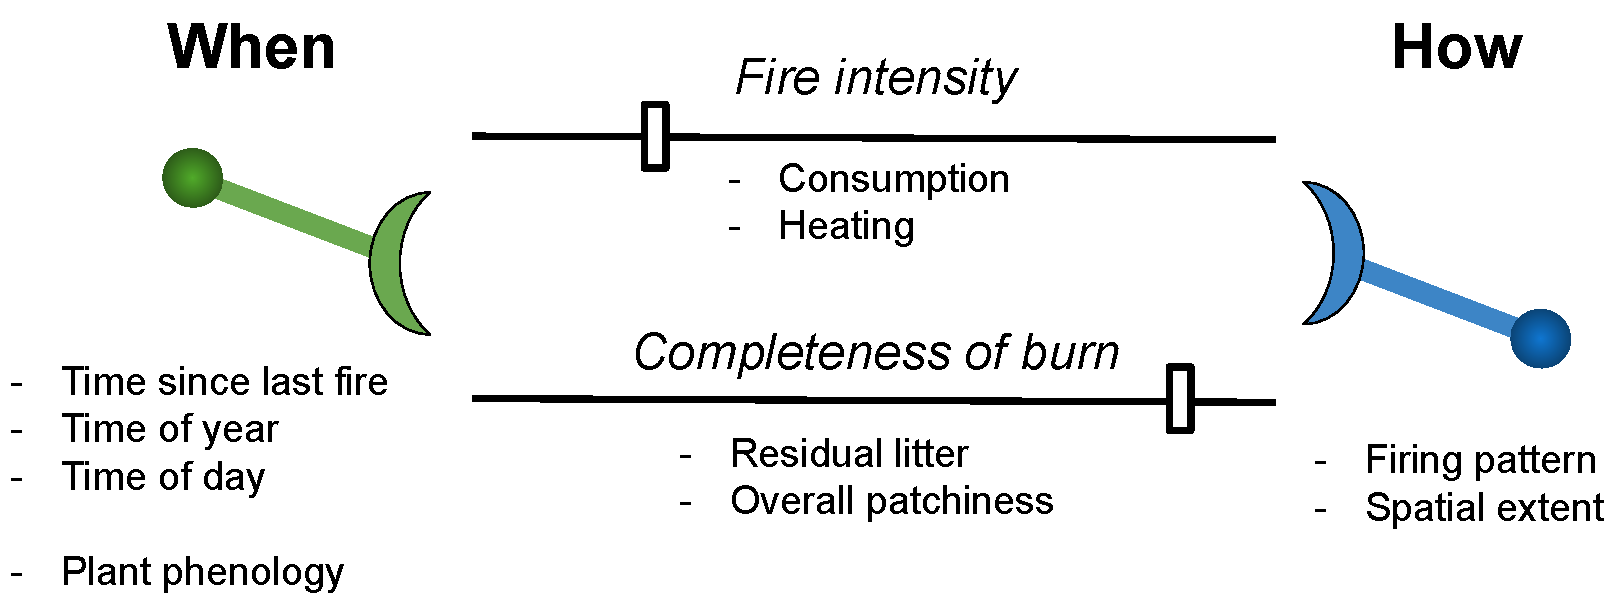
\includegraphics[width=1\linewidth]{figs/levers} 
		\end{figure}
	\end{center}
\alert{Great Plains are in a \textbf{fire deficit} and management is best focused on \textbf{burning new acres}}
\end{frame}



\begin{frame}{Mopping up} 

\begin{columns}
\begin{column}{0.55\textwidth}
\begin{itemize}
	\item Fight the deficit: Burn what you can, when you can, but try to add new acres
	\item[]
		\item Focus on fine-scale levers to accomplish objectives regardless of season
	\item[]
	\item Consider emphasis on burn completeness: \emph{defend desired refugia}

\end{itemize}
\end{column}
\begin{column}{0.5\textwidth}  
\begin{center}
\begin{figure}
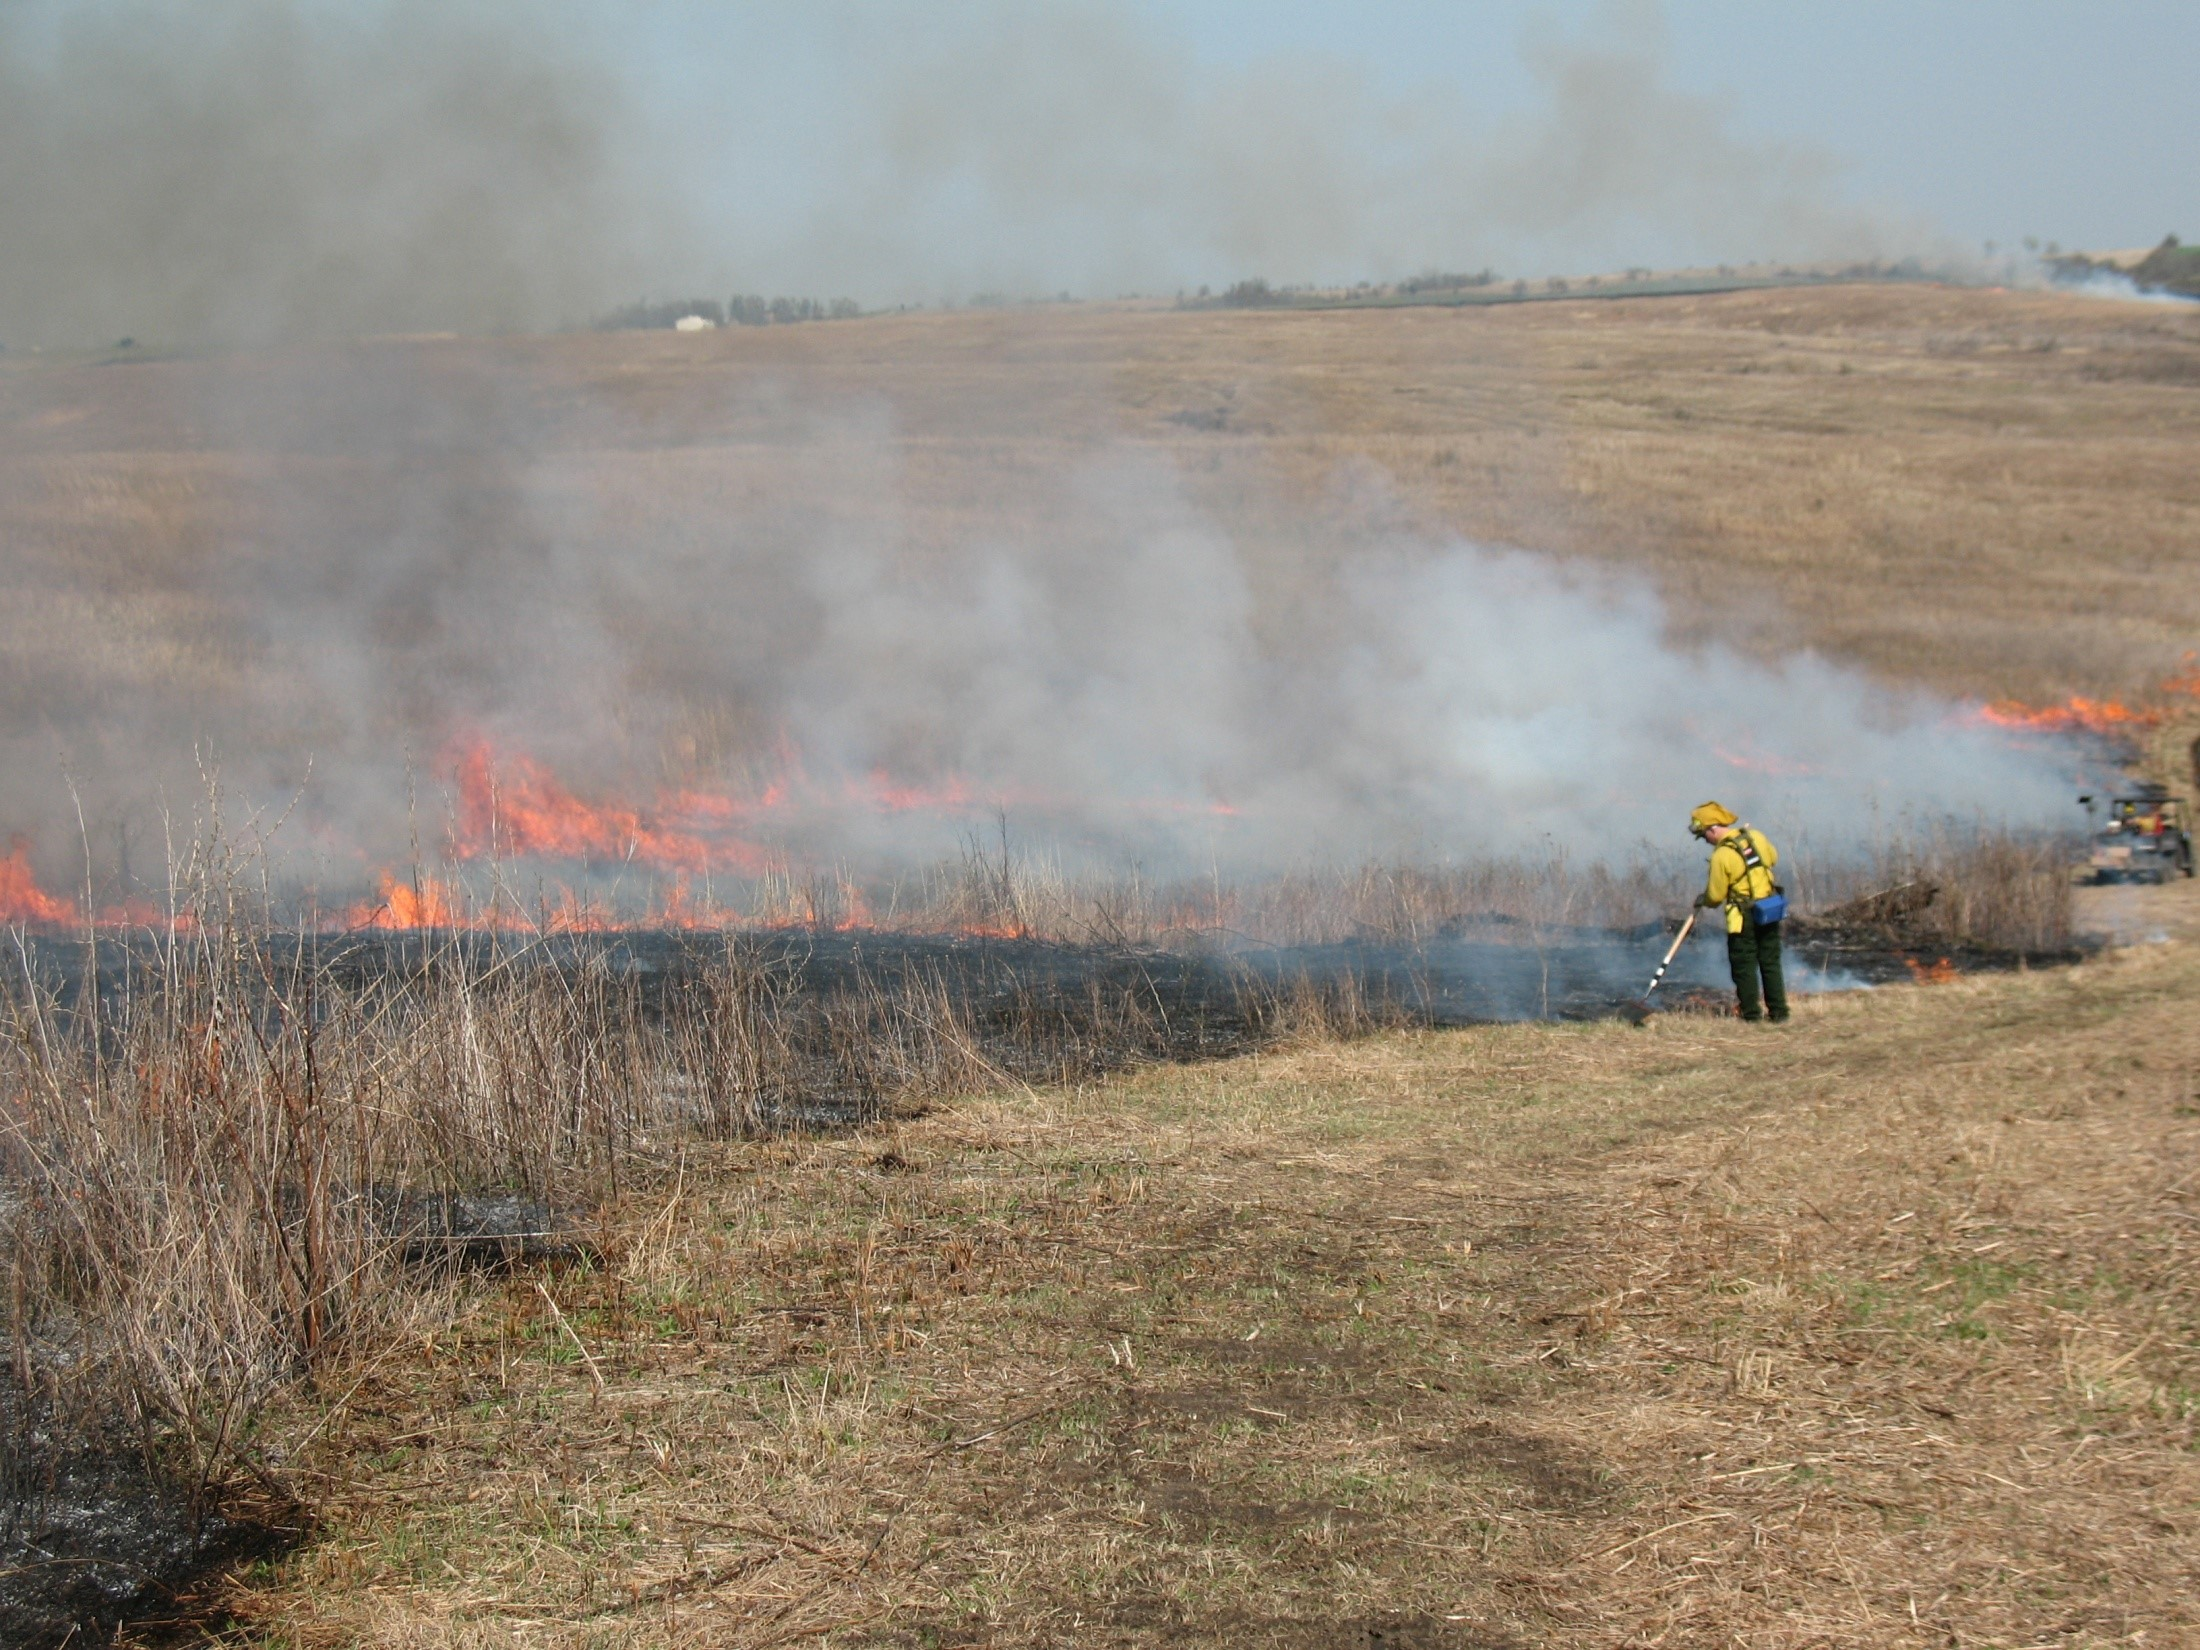
\includegraphics[width=1\linewidth]{figs/mop_up} 
 \end{figure}
\end{center}
\end{column}
\end{columns}
\end{frame}

\begin{frame}{Thank you!}
Any questions before you all run away?
\begin{center}
\begin{figure}
 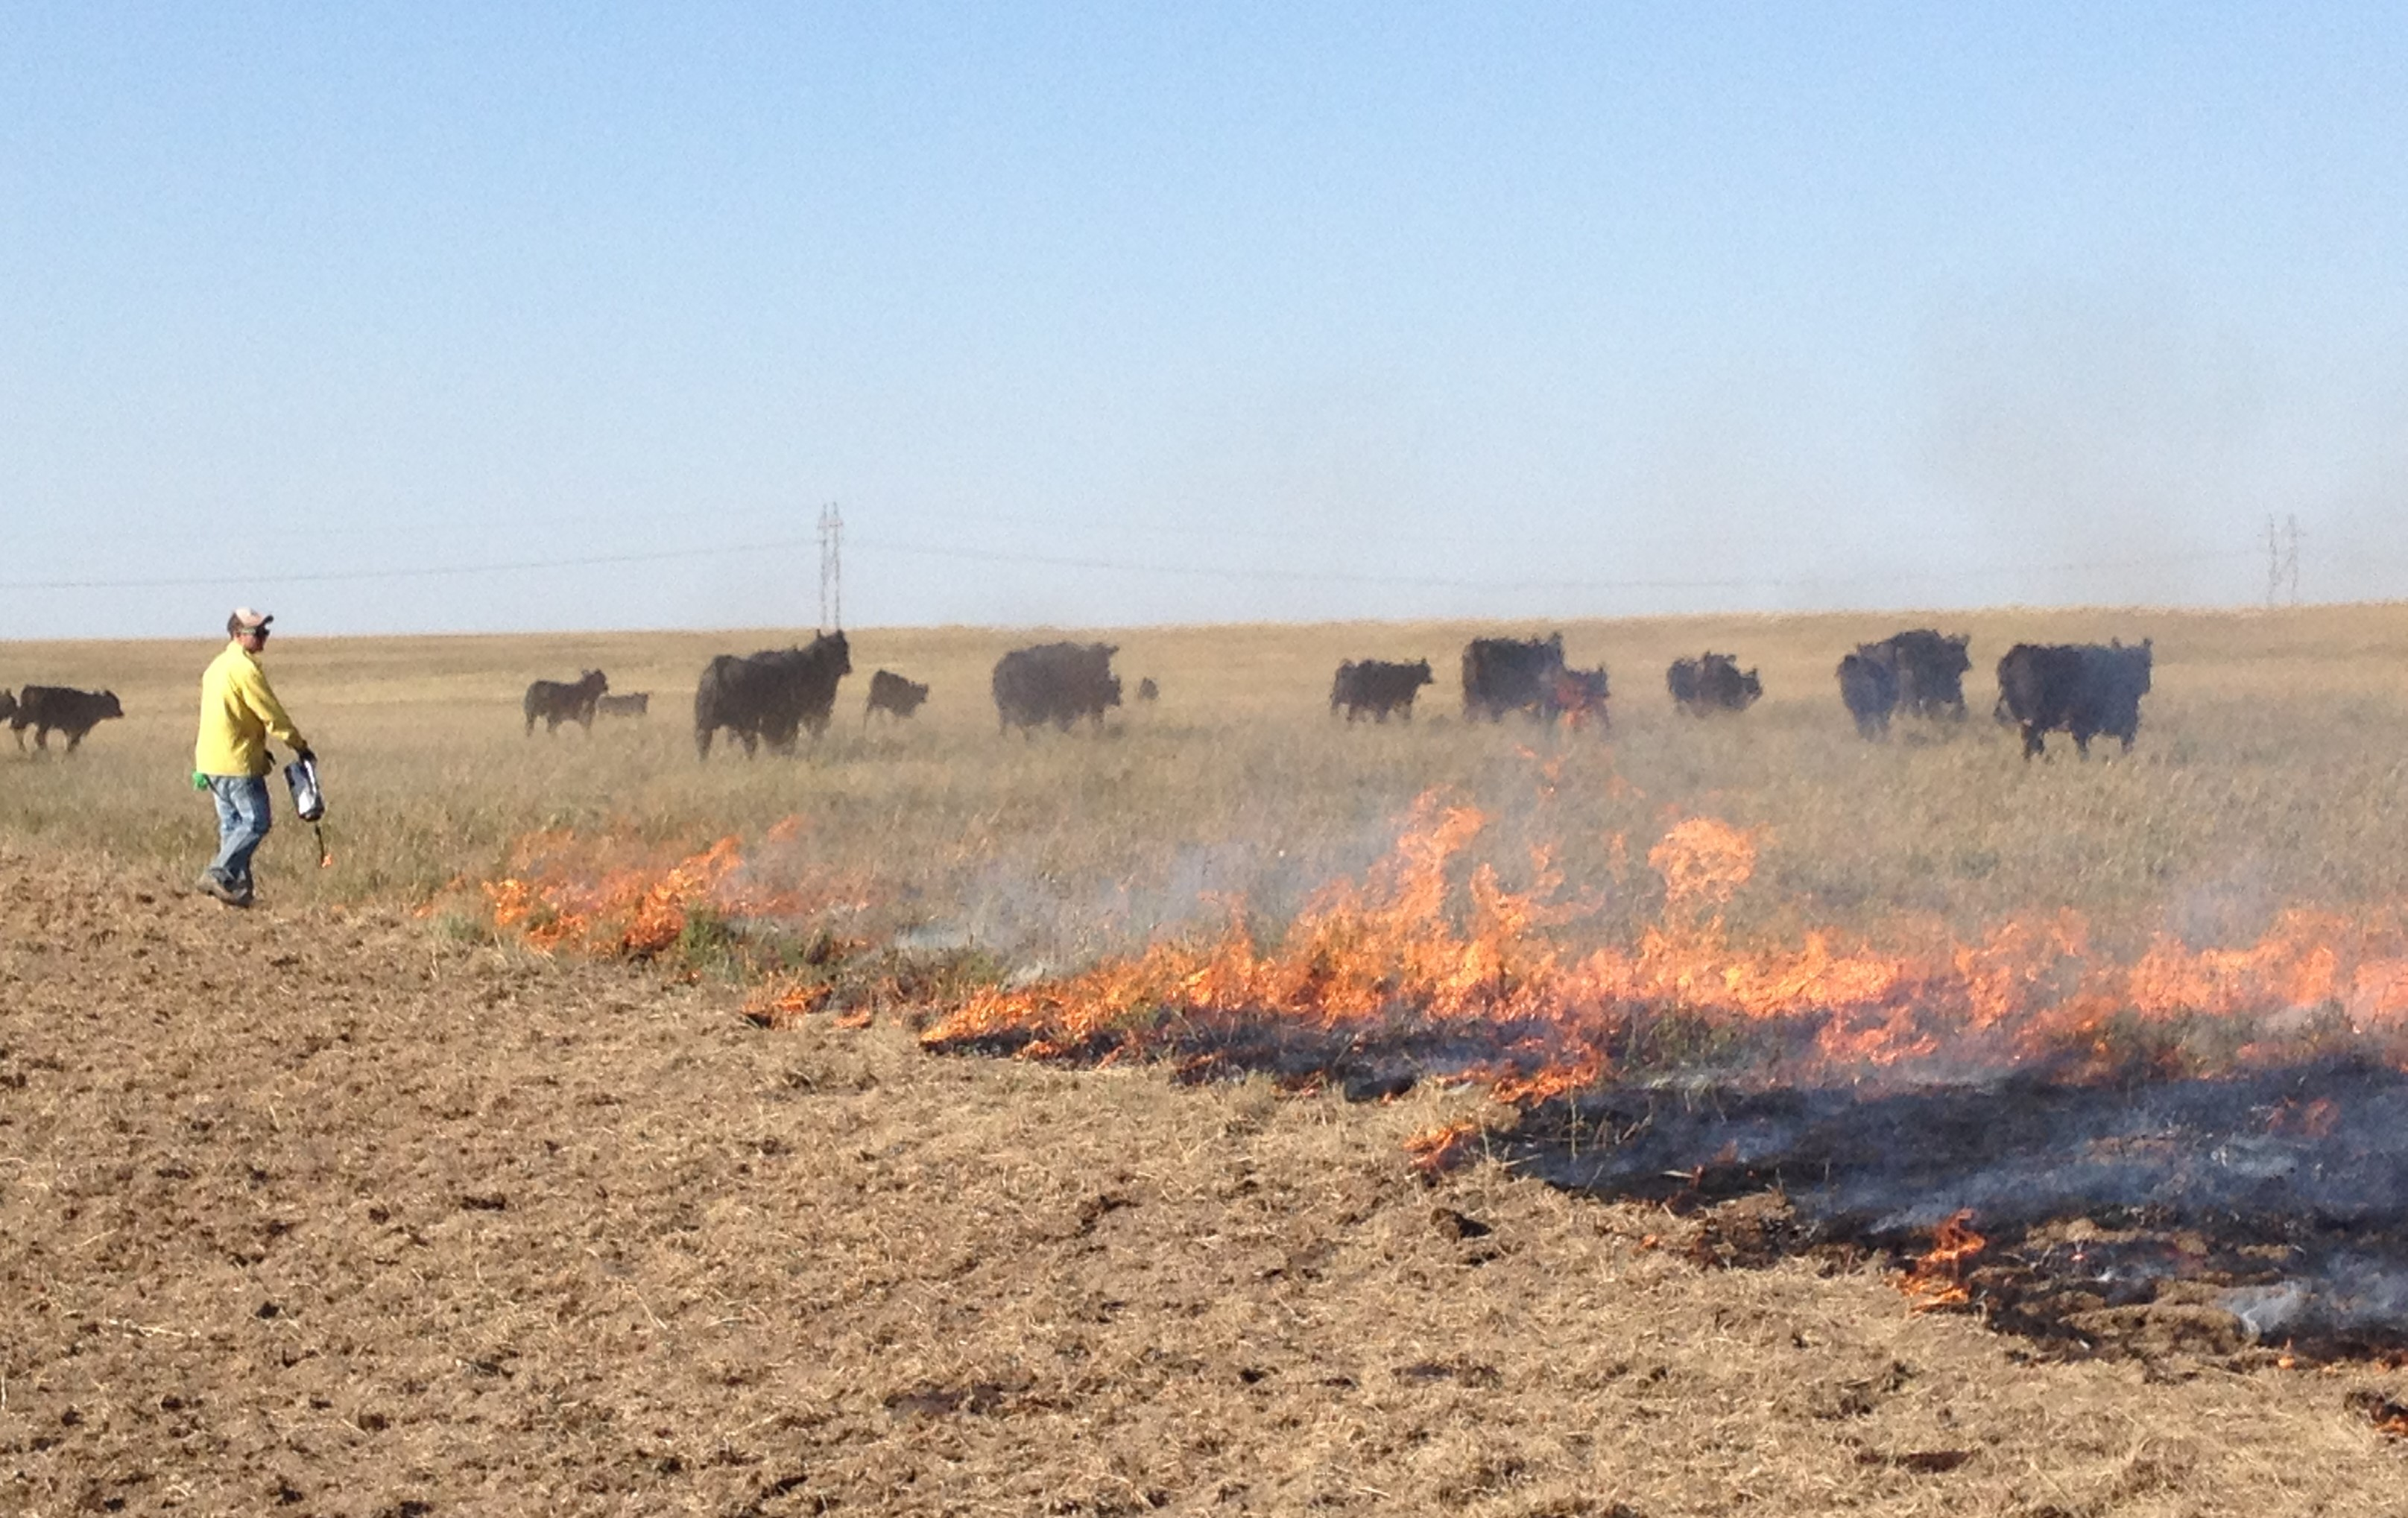
\includegraphics[width=1\linewidth]{figs/fire_cows_close} 

 \end{figure}
\end{center}
\end{frame}

\end{document}
